\appendix

\section{Figures}
Since we could not fit all figures in eight pages, we include them here.

\begin{figure}[h!]
  \centering
  \begin{subfigure}[b]{0.45\textwidth}
    \centering
    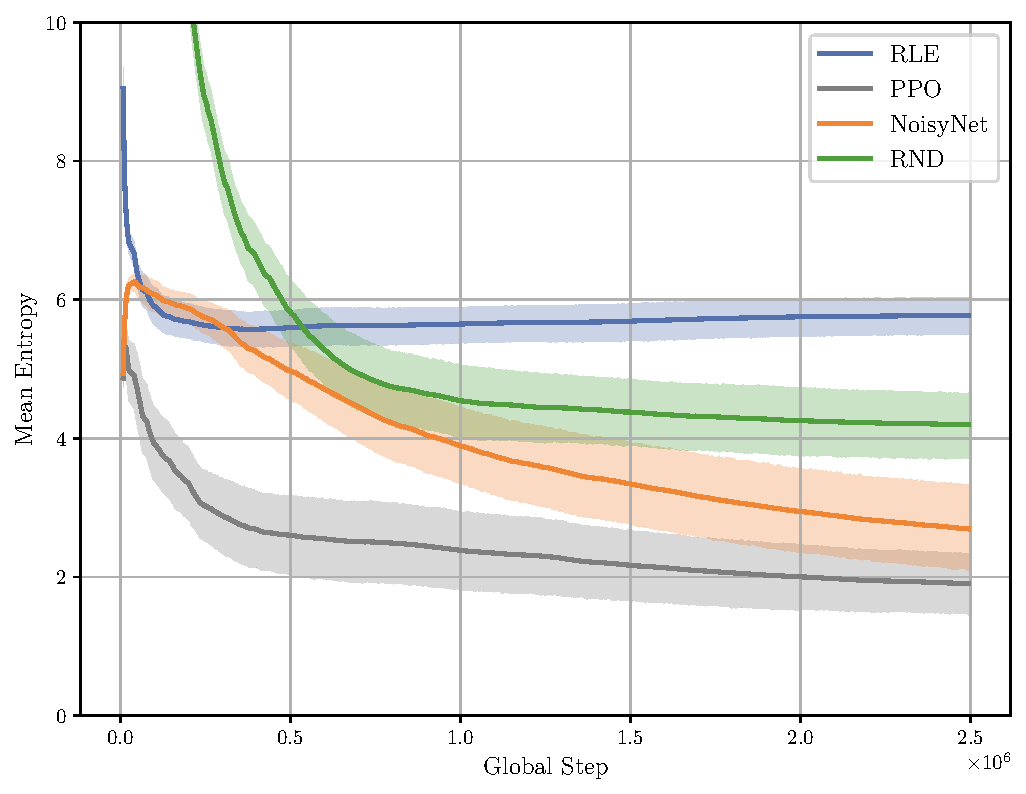
\includegraphics[width=\textwidth]{figures/gridworld_mean_entropy_state_visitation_algorithms.pdf}
    \caption{Mean entropy of state visitation counts over the training steps for different algorithms. The shaded areas represent the $95\%$ confidence intervals. By the end of training, \textsc{RLE} achieves the highest entropy and the narrowest confidence interval.}
    \label{fig:gridworld-entropy-algorithms}
  \end{subfigure}
  \hfill
  \begin{subfigure}[b]{0.45\textwidth}
    \centering
    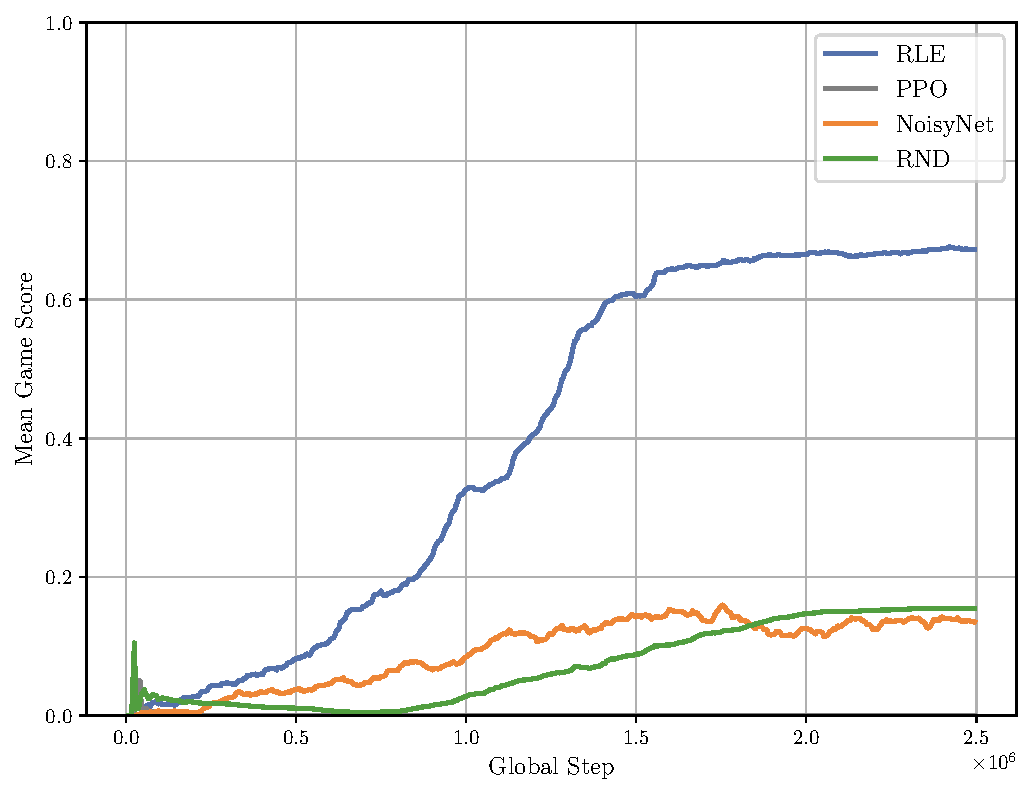
\includegraphics[width=\textwidth]{figures/gridworld_mean_game_score_algorithms.pdf}
    \caption{Mean game score of different algorithms. \textsc{RLE} clearly outperforms the other algorithms.\\\\}
    \label{fig:gridworld-score-algorithms}
  \end{subfigure}
  \begin{subfigure}[b]{0.45\textwidth}
    \centering
    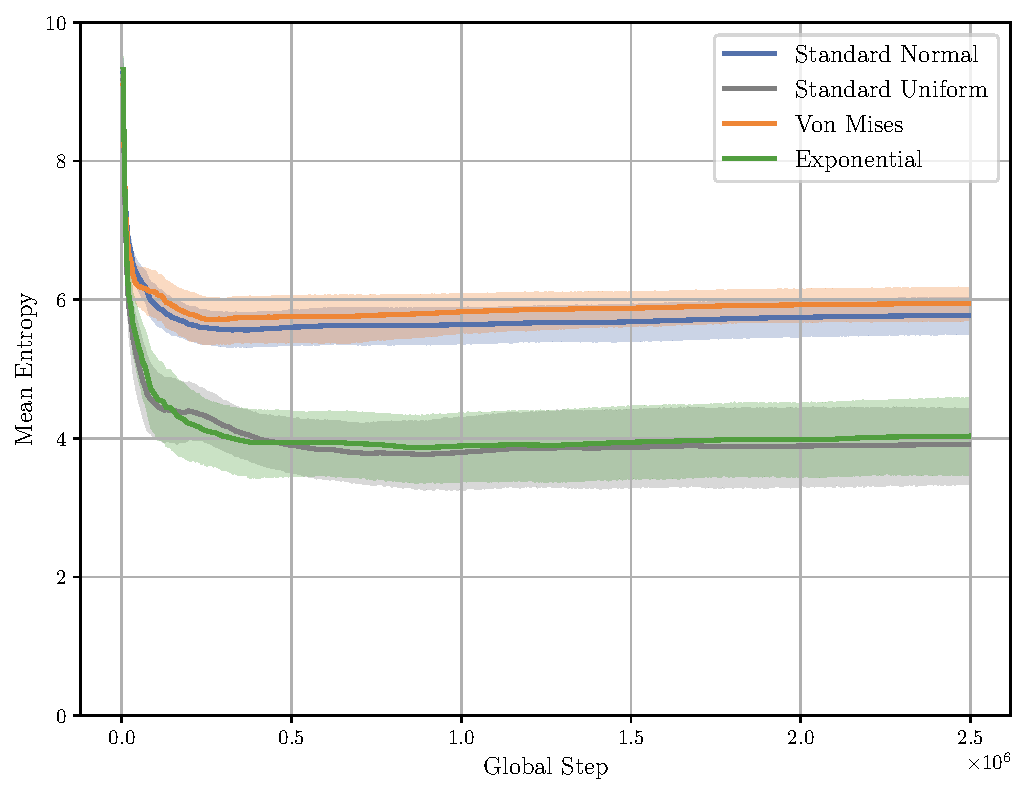
\includegraphics[width=\textwidth]{figures/gridworld_mean_entropy_state_visitation_distributions.pdf}
    \caption{Mean entropy of state visitation counts over the training steps for \textsc{RLE} variants with different latent vector distributions. The shaded areas represent the $95\%$ confidence intervals. The standard uniform and exponential variants explore less than the other two variants.}
    \label{fig:gridworld-entropy-distributions}
  \end{subfigure}
  \hfill
  \begin{subfigure}[b]{0.45\textwidth}
    \centering
    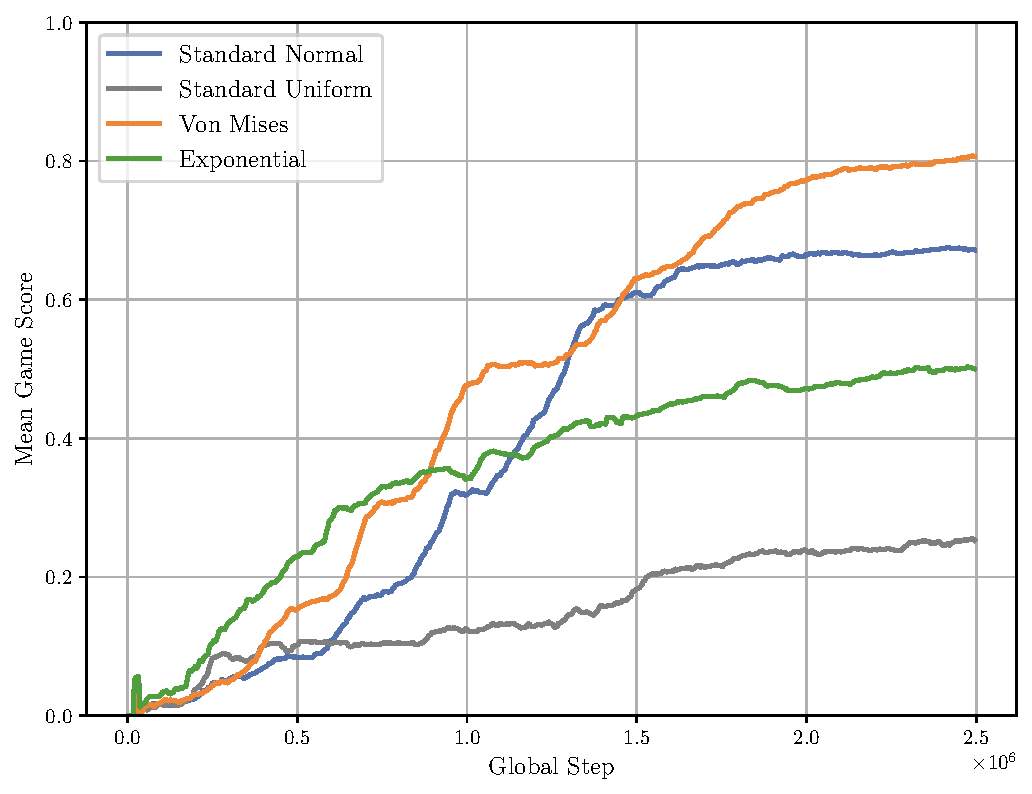
\includegraphics[width=\textwidth]{figures/gridworld_mean_game_score_distributions.pdf}
    \caption{Mean game score of \textsc{RLE} variants with different latent vector distributions. The figure shows substantial differences in the mean game score across the different \textsc{RLE} variants.\\\\}
    \label{fig:gridworld-score-distributions}
  \end{subfigure}
  \caption{\textsc{FourRoom} results.}
  \label{fig:gridworld-plots}
\end{figure}

\clearpage
\begin{figure}[h!]
  \centering
  \begin{subfigure}[b]{0.45\textwidth}
    \centering
    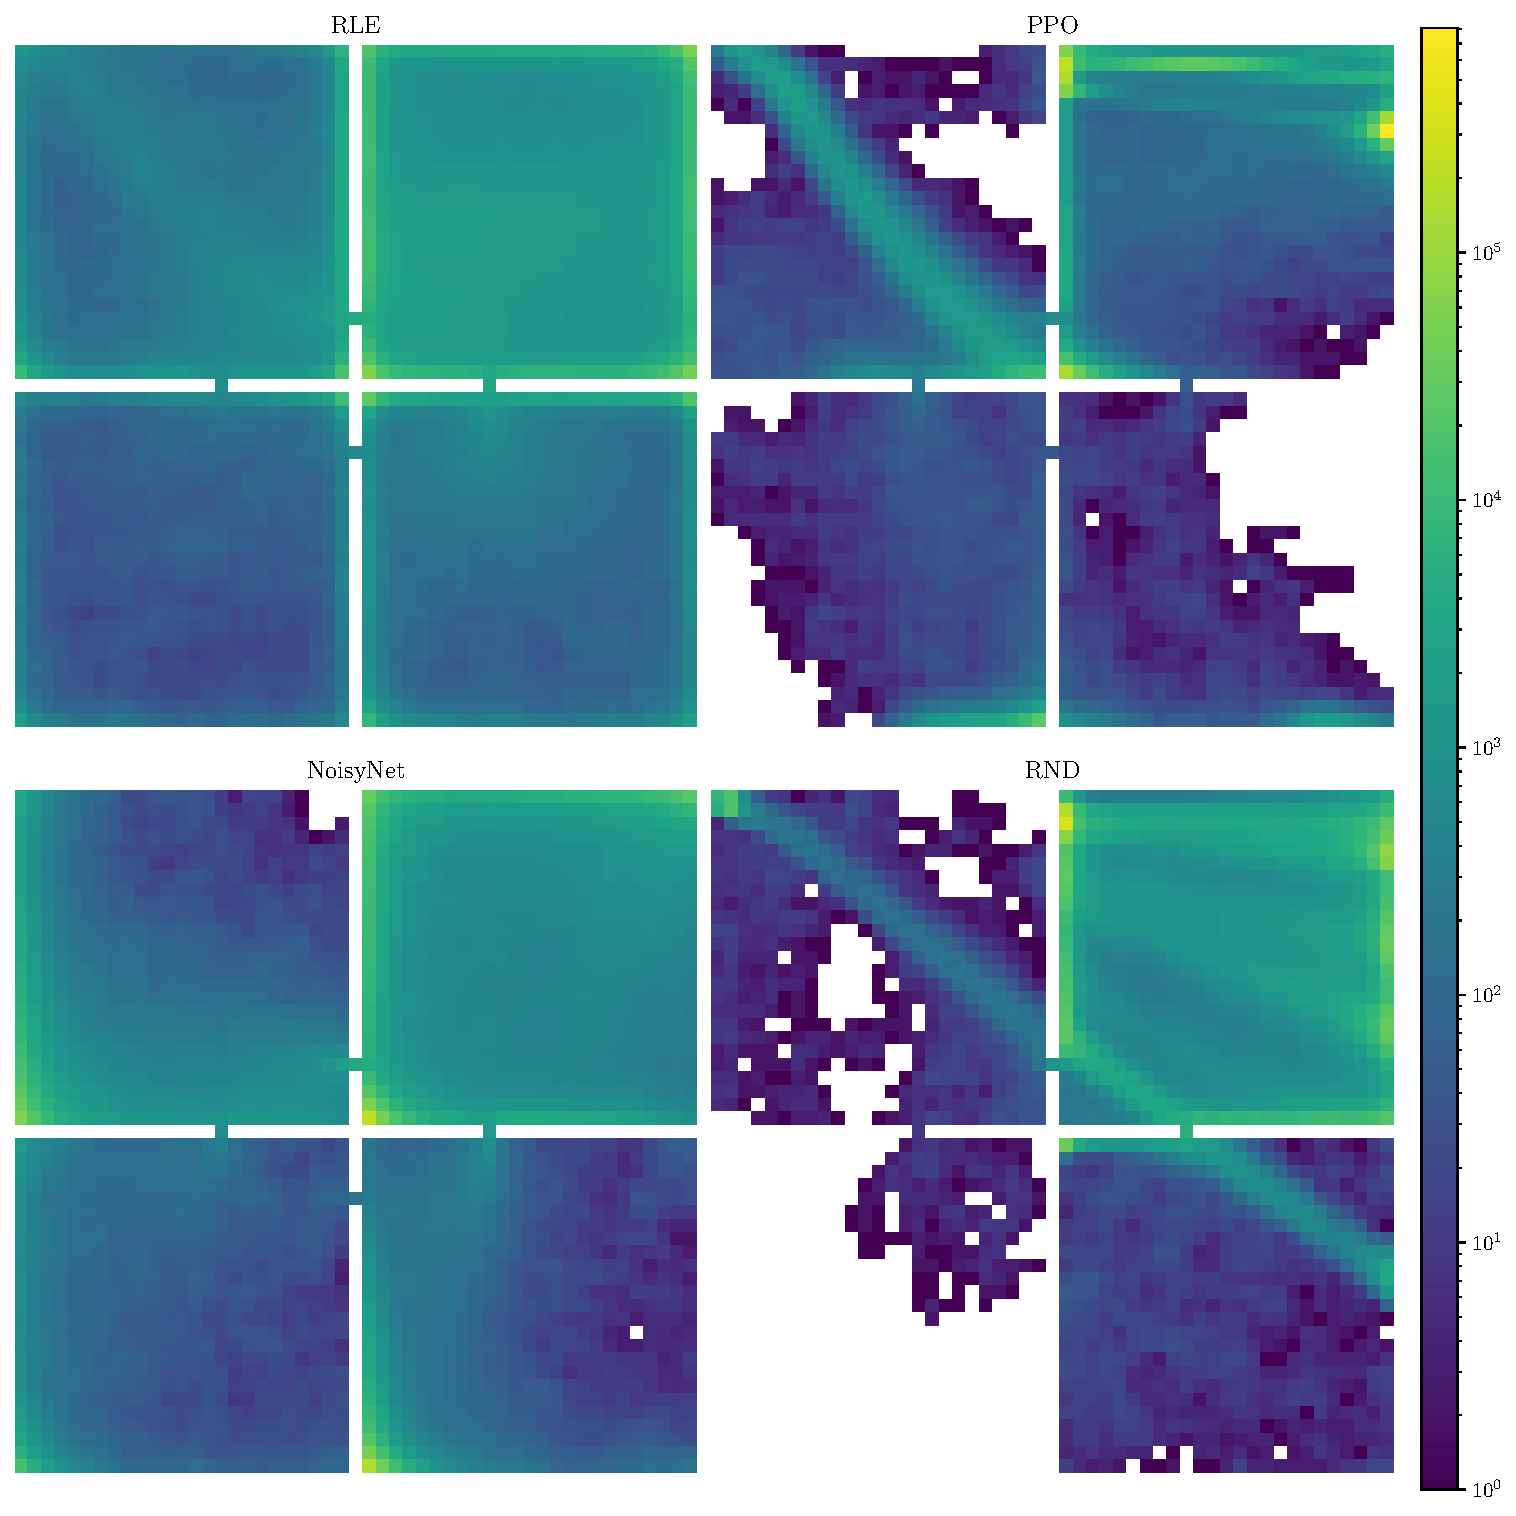
\includegraphics[width=\textwidth]{figures/gridworld_heatmaps_no_goal_algorithms.pdf}
    \caption{For each algorithm, the run with the highest entropy over the state visitation counts was selected to generate the heatmap. The heatmap illustrates the state visitation counts of all the algorithms after training for $2.5$M timesteps in the reward-free environment. The start location is in the top right cell. \textsc{RLE} achieves the best state visitation coverage.}
    \label{fig:gridworld-heatmap-nogoal-algorithms}
  \end{subfigure}
  \hfill
  \begin{subfigure}[b]{0.45\textwidth}
    \centering
    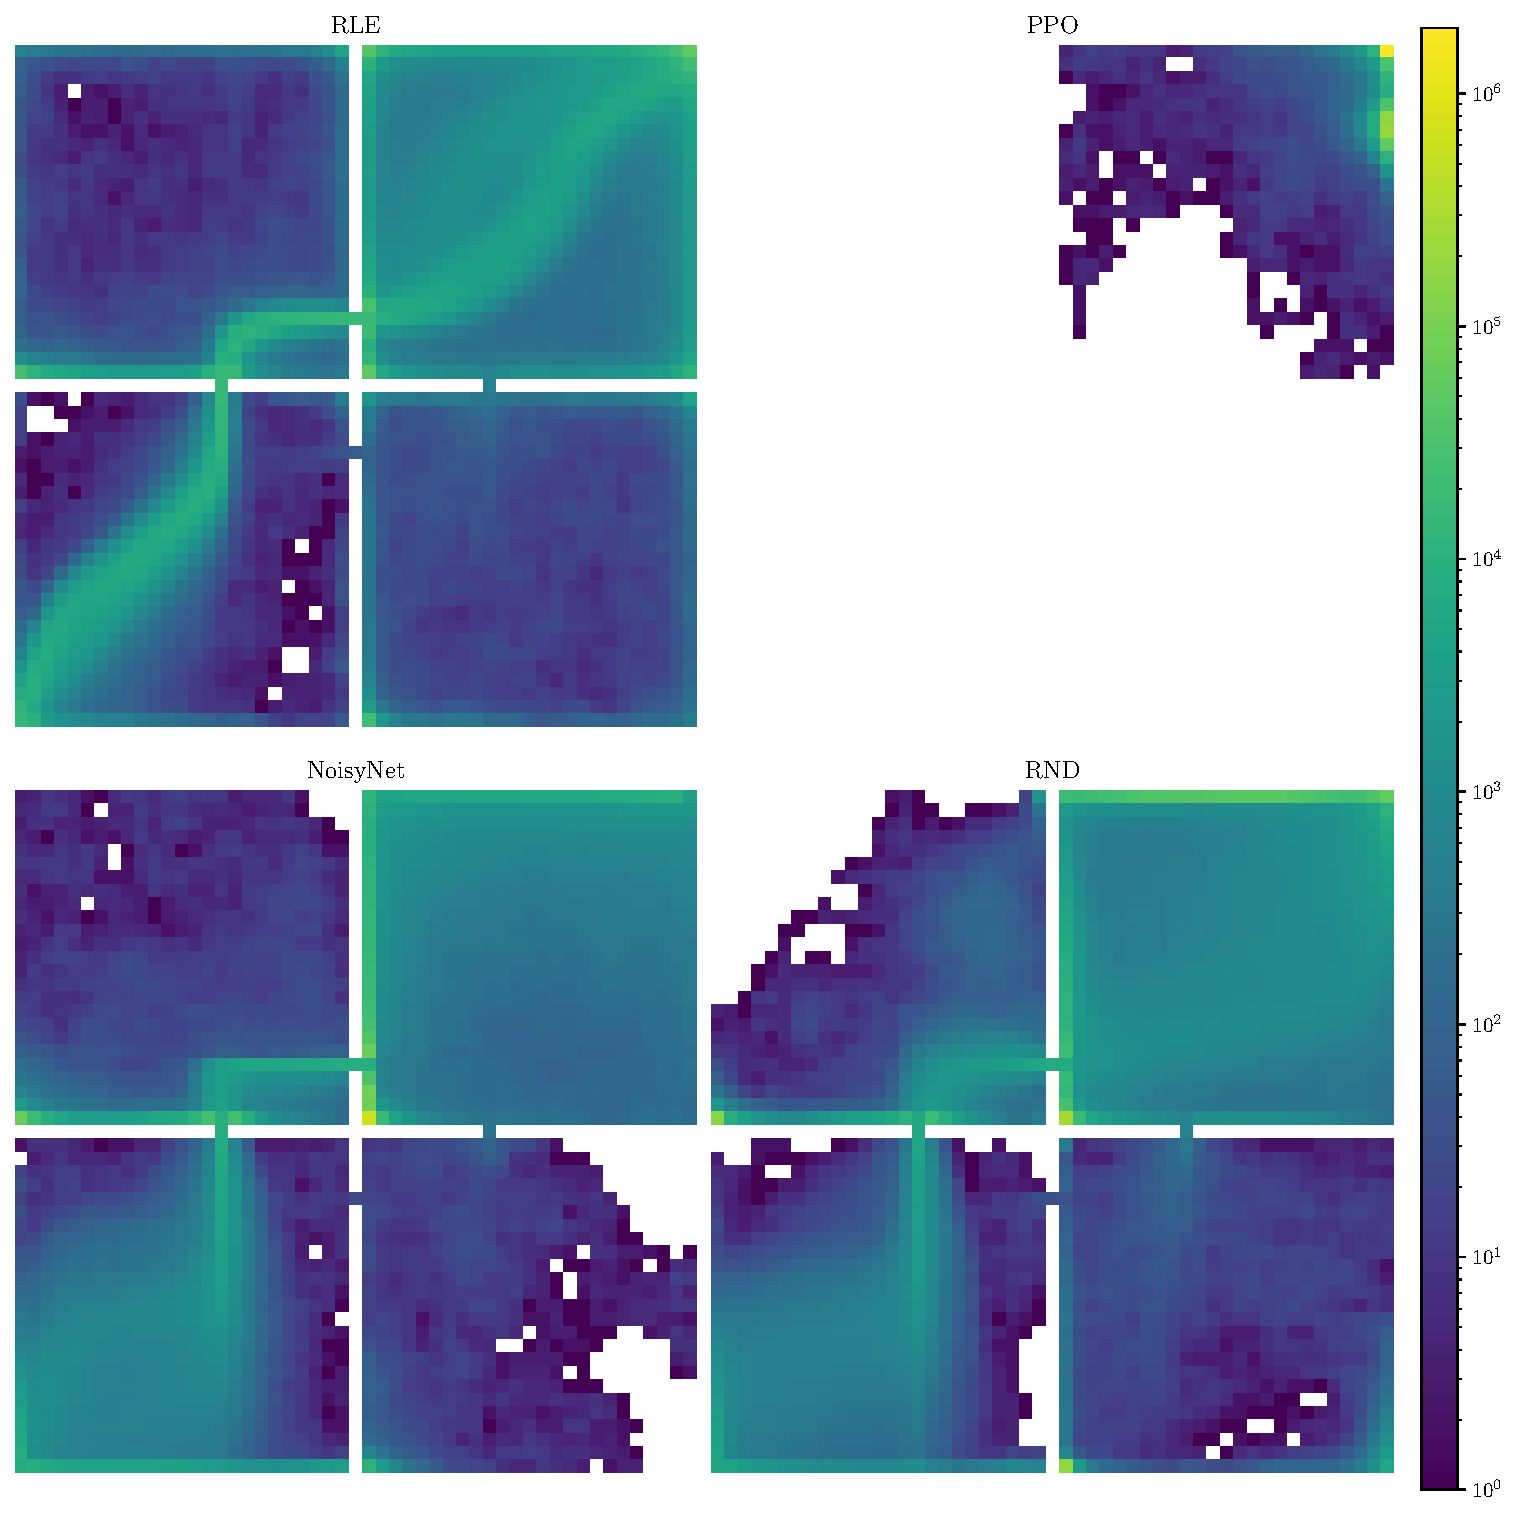
\includegraphics[width=\textwidth]{figures/gridworld_heatmaps_goal_algorithms.pdf}
    \caption{For each algorithm, the run with the highest game score was selected to generate the heatmap. The heatmap illustrates the state visitation counts of all the algorithms after training for $2.5$M timesteps in the environment with a goal. The start location is in the top right cell and the goal location in the bottom left cell.}
    \label{fig:gridworld-heatmap-goal-algorithms}
  \end{subfigure}
  \begin{subfigure}[b]{0.45\textwidth}
    \centering
    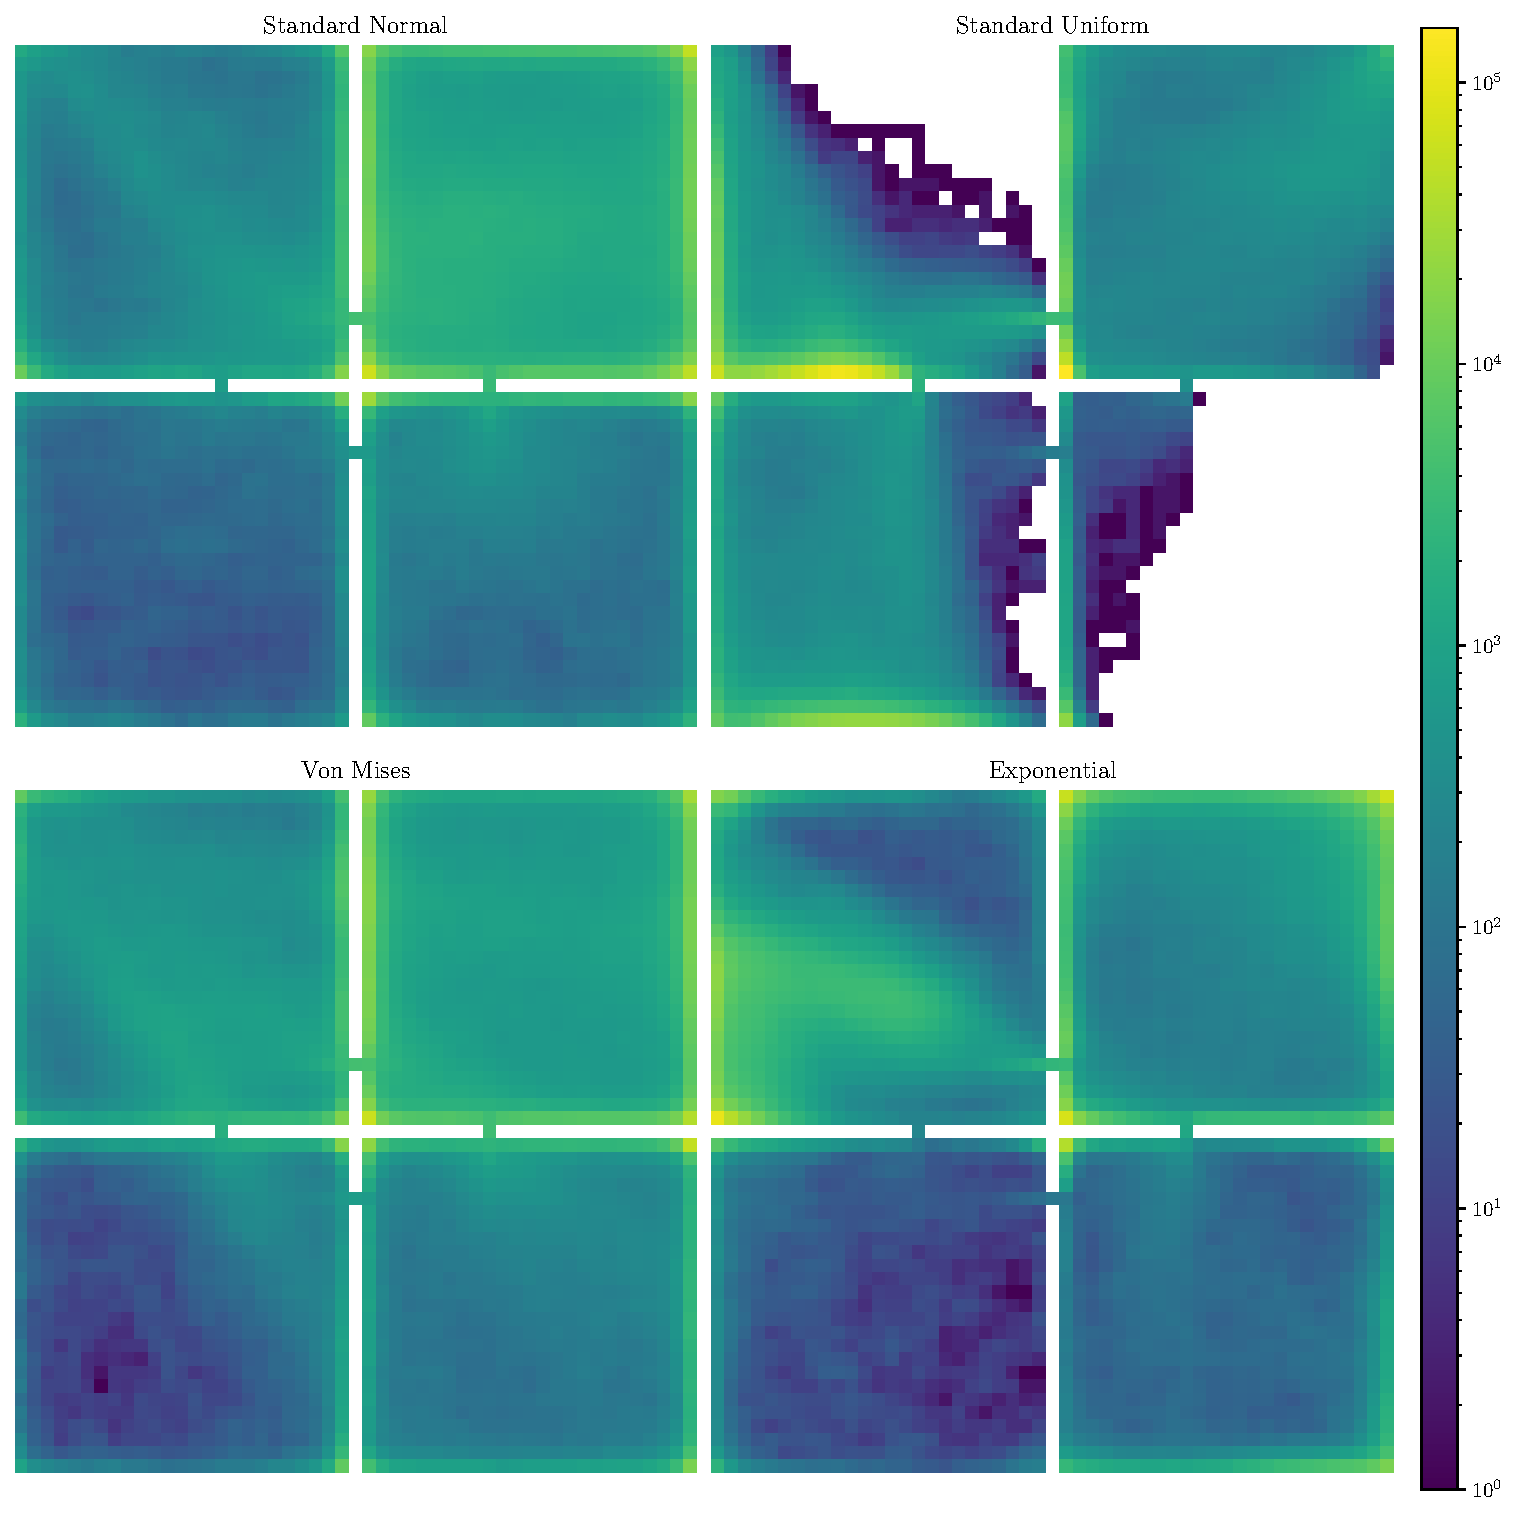
\includegraphics[width=\textwidth]{figures/gridworld_heatmaps_no_goal_distributions.pdf}
    \caption{For each \textsc{RLE} variant with different latent vector distribution, the run with the highest entropy over the state visitation counts was selected to generate the heatmap. The heatmap illustrates the state visitation counts of all the \textsc{RLE} variants with different latent vector distribution after training for $2.5$M timesteps in the reward-free environment. The \textsc{RLE} variants where the latent vector distribution is a standard normal and the Von Mises distribution achieve the best state visitation coverage.}
    \label{fig:gridworld-heatmap-nogoal-distributions}
  \end{subfigure}
  \hfill
  \begin{subfigure}[b]{0.45\textwidth}
    \centering
    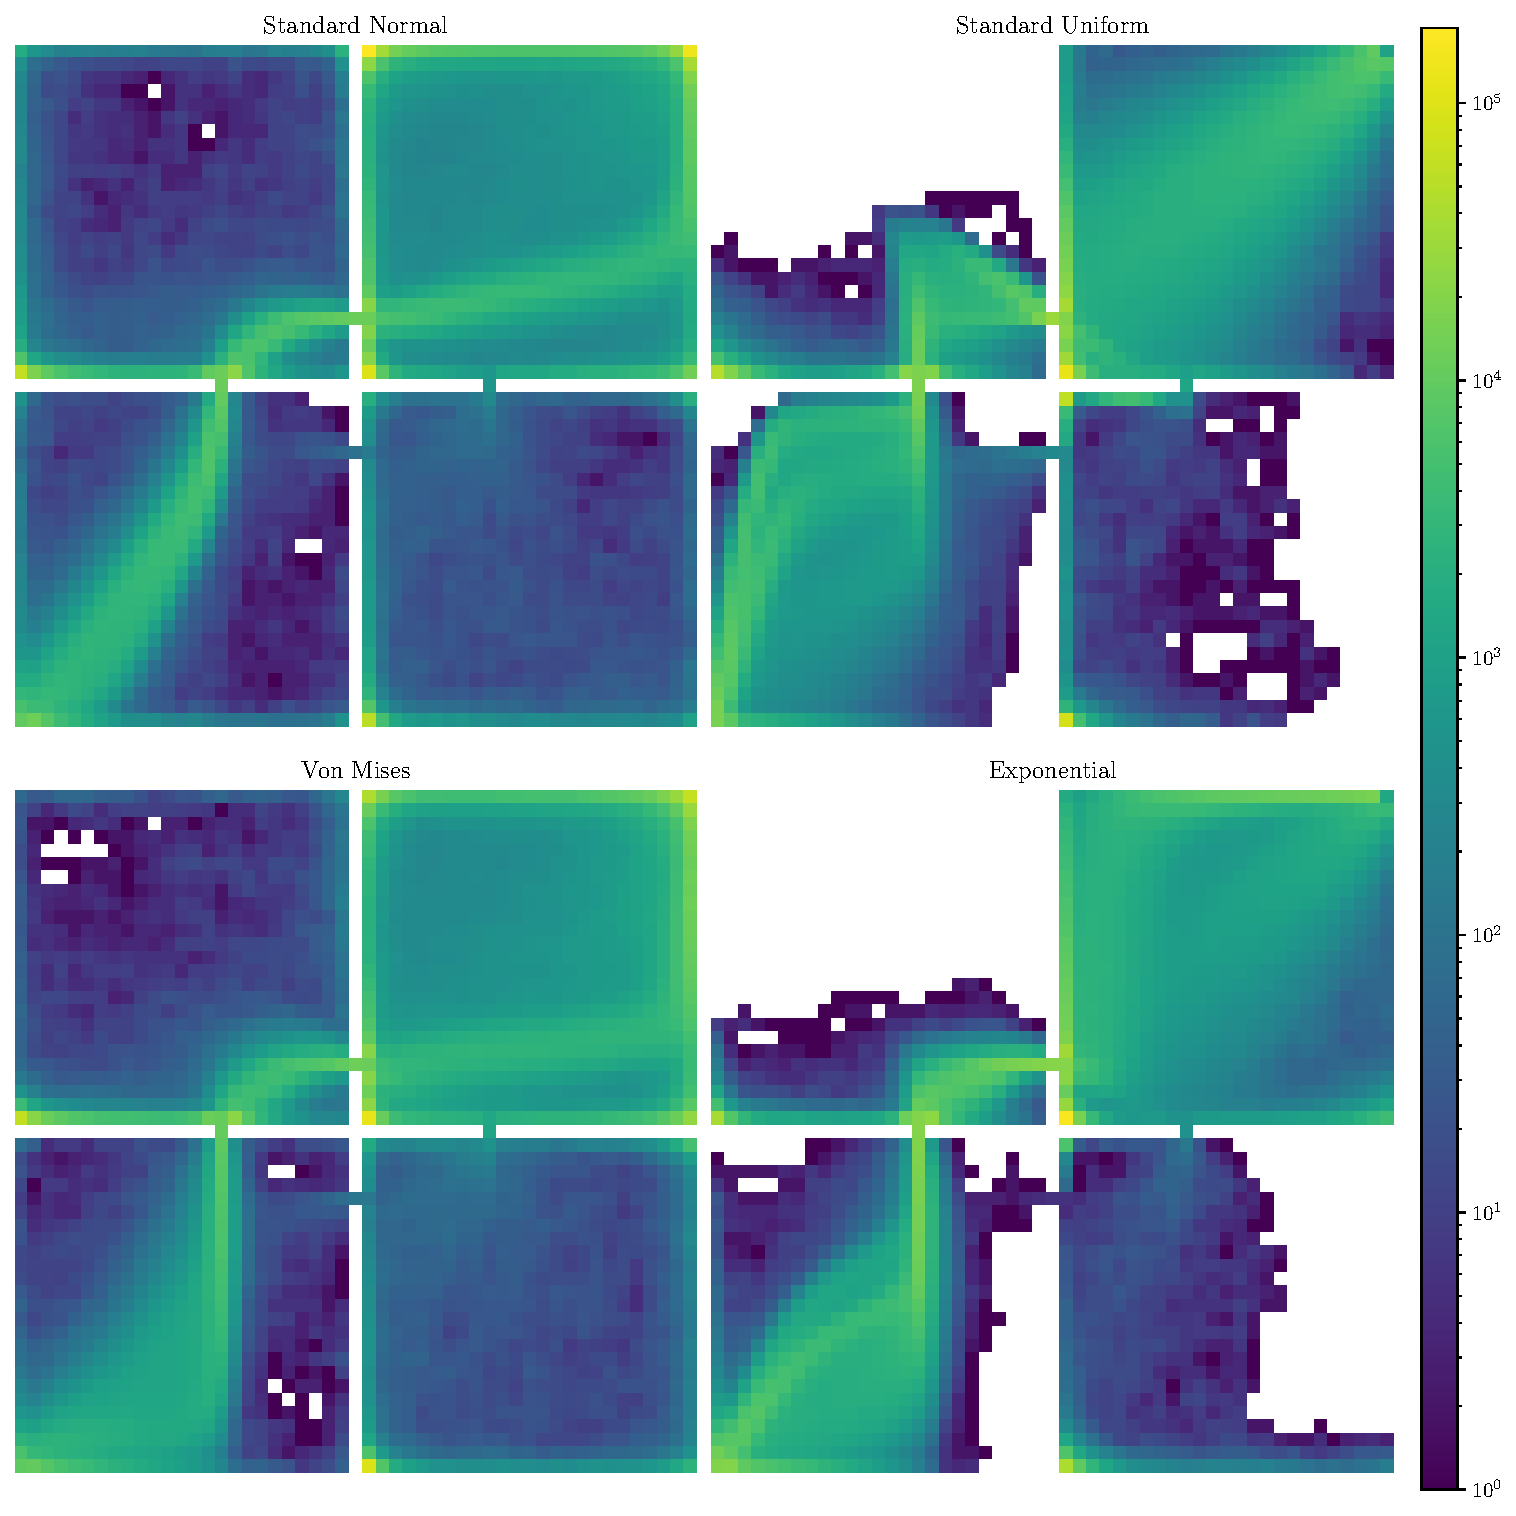
\includegraphics[width=\textwidth]{figures/gridworld_heatmaps_goal_distributions.pdf}
    \caption{For each \textsc{RLE} variant with different latent vector distribution, the run with the highest game score was selected to generate the heatmap. The heatmap illustrates the state visitation counts of all the \textsc{RLE} variants with different latent vector distribution after training for $2.5$M timesteps in the environment with a goal. The start location is in the top right cell and the goal location in the bottom left cell. All \textsc{RLE} variants reach the goal but the standard normal and Von Mises variants also explore most of the state space.}
    \label{fig:gridworld-heatmap-goal-distributions}
  \end{subfigure}
  \caption{\textsc{FourRoom} state visitation heatmaps.}
  \label{fig:gridworld-statemaps}
\end{figure}

\begin{figure}[h!]
  \centering
  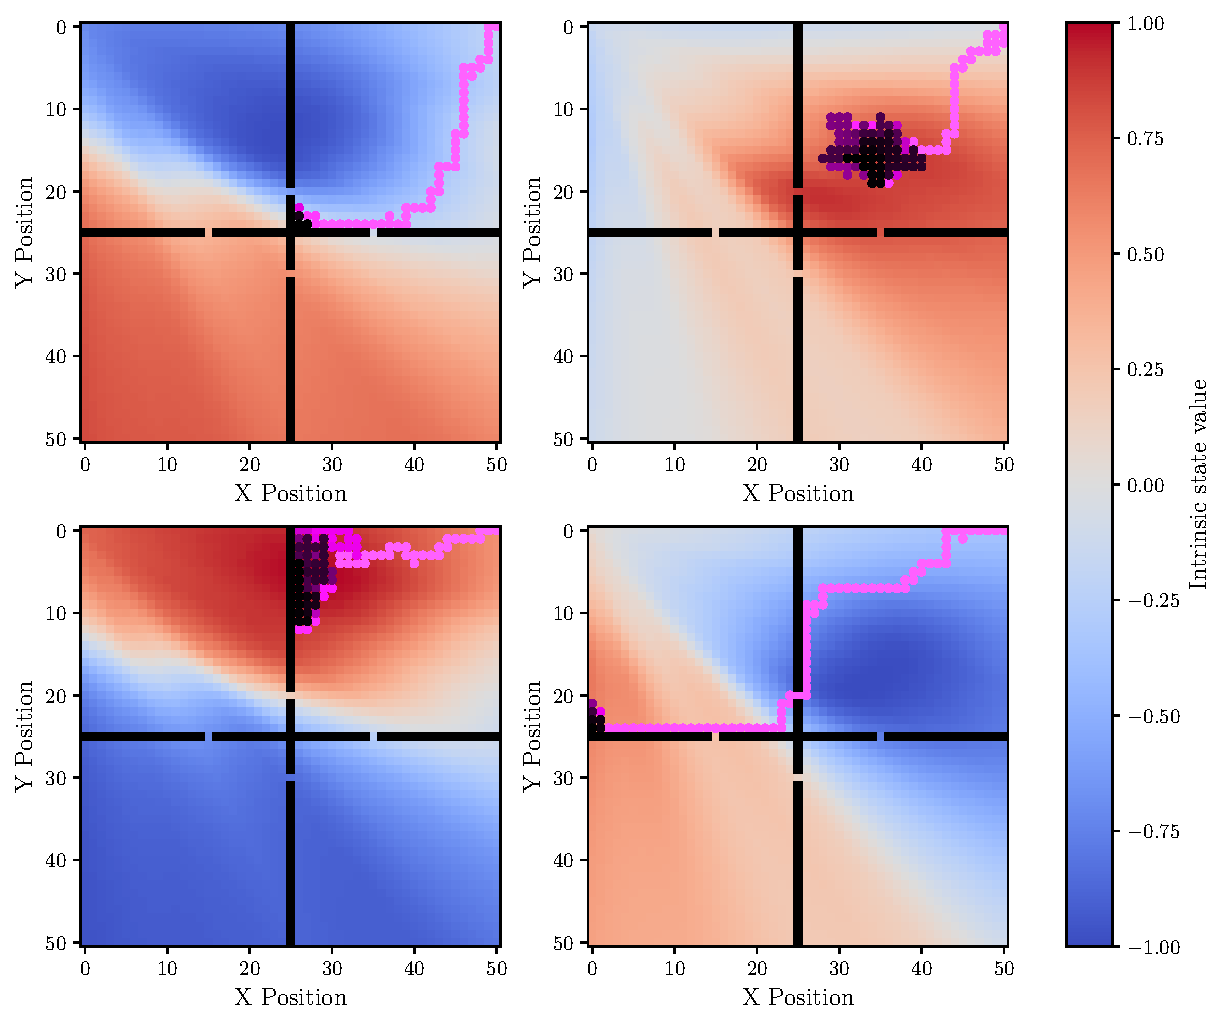
\includegraphics[width=0.6\textwidth]{figures/gridworld_value_function_trajectory.pdf}
  \caption{Trajectory and intrinsic reward function for four different $\textbf{z}$ values. Earlier steps in the trajectory are pink and with increasing number of steps the color shifts to black. The trajectories generally tend towards regions with high intrinsic reward. The example is not cherry-picked. This behavior was observed for almost every figure we generated.}
  \label{fig:gridworld-value-function-trajectories}
\end{figure}

\begin{figure}[h!]
  \centering
  \begin{subfigure}[b]{0.45\textwidth}
    \centering
    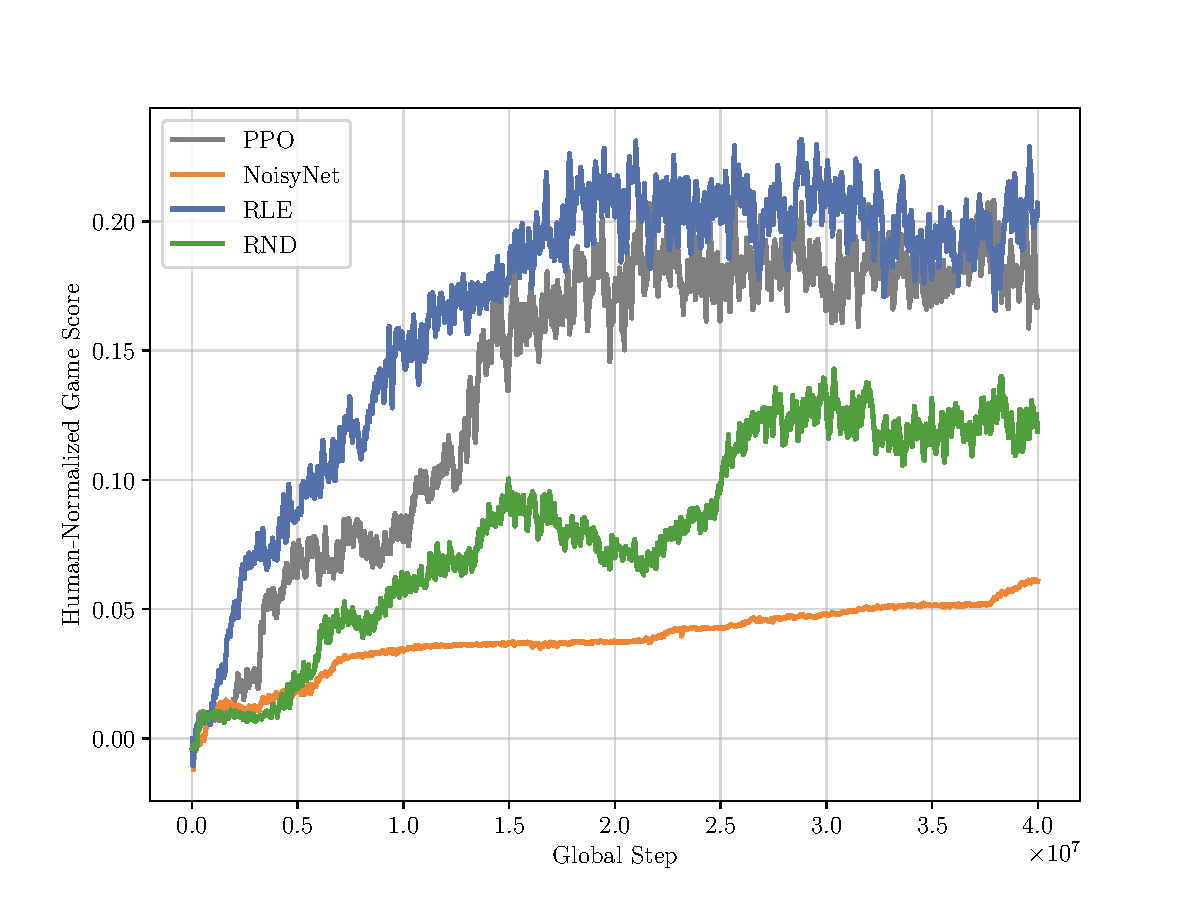
\includegraphics[width=\textwidth]{figures/plot_Alien_Score.pdf}
    \caption{Game Score.}
    \label{fig:alien-score}
  \end{subfigure}
  \hfill
  \begin{subfigure}[b]{0.45\textwidth}
    \centering
    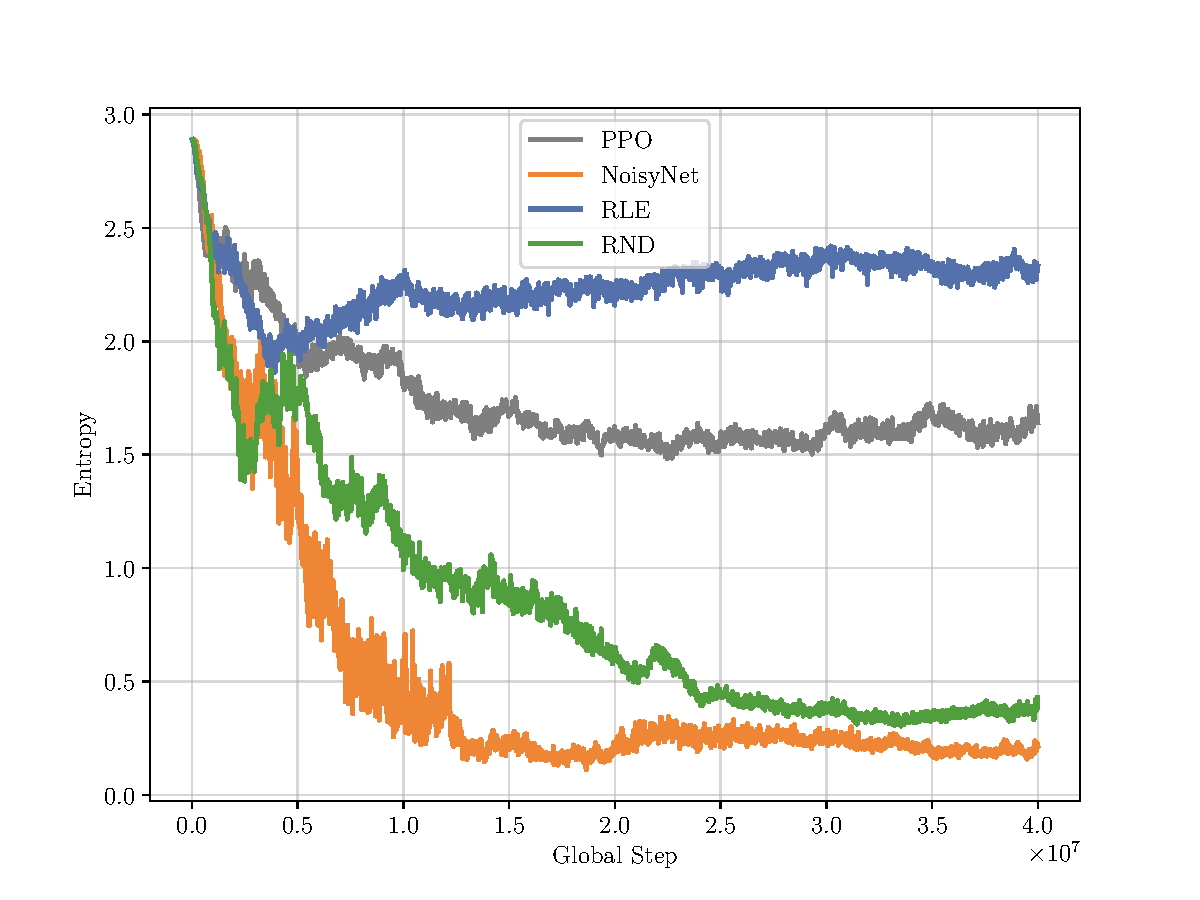
\includegraphics[width=\textwidth]{figures/plot_Alien_Entropy.pdf}
    \caption{Entropy.}
    \label{fig:alien-entropy}
  \end{subfigure}
  \begin{subfigure}[b]{0.45\textwidth}
    \centering
    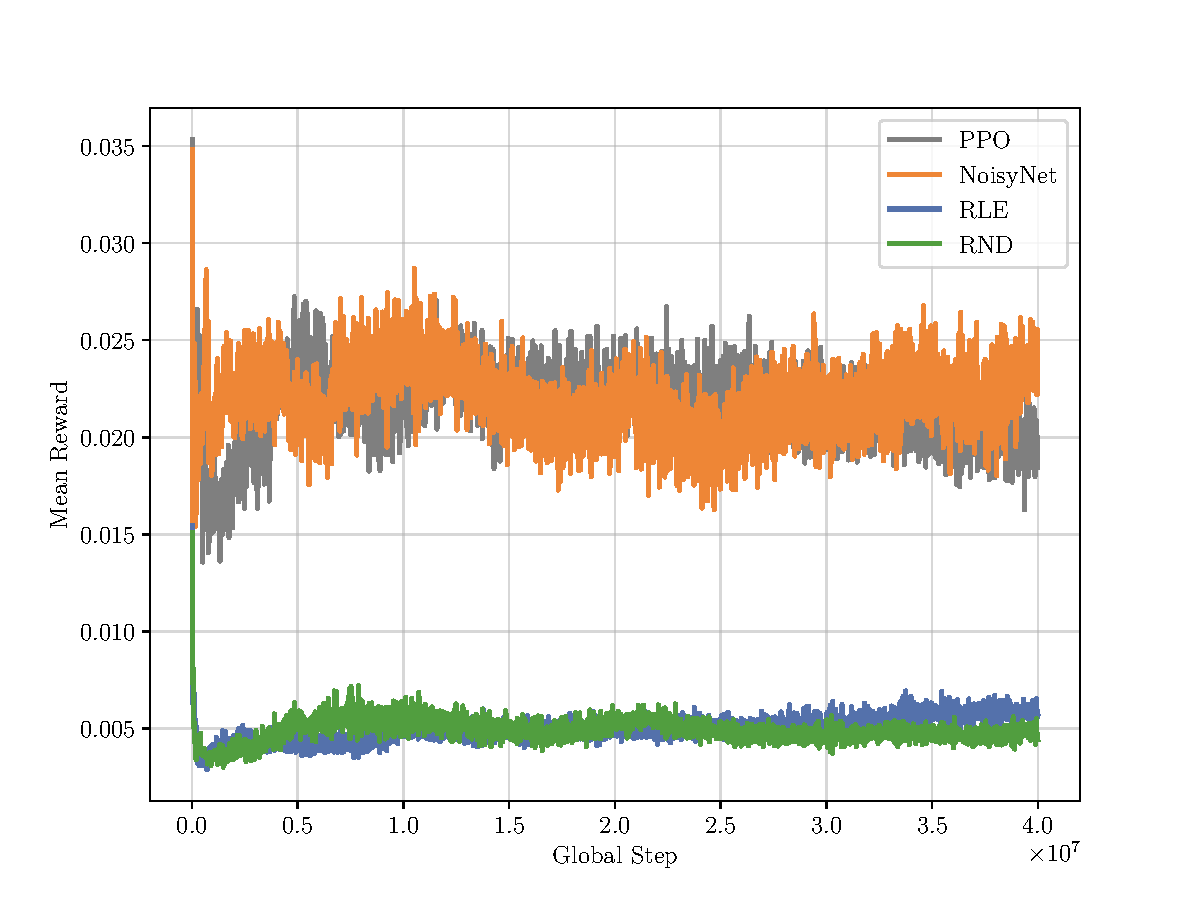
\includegraphics[width=\textwidth]{figures/plot_Alien_RewardsMean.pdf}
    \caption{Mean Reward.}
    \label{fig:alien-rewards}
  \end{subfigure}
  \hfill
  \begin{subfigure}[b]{0.45\textwidth}
    \centering
    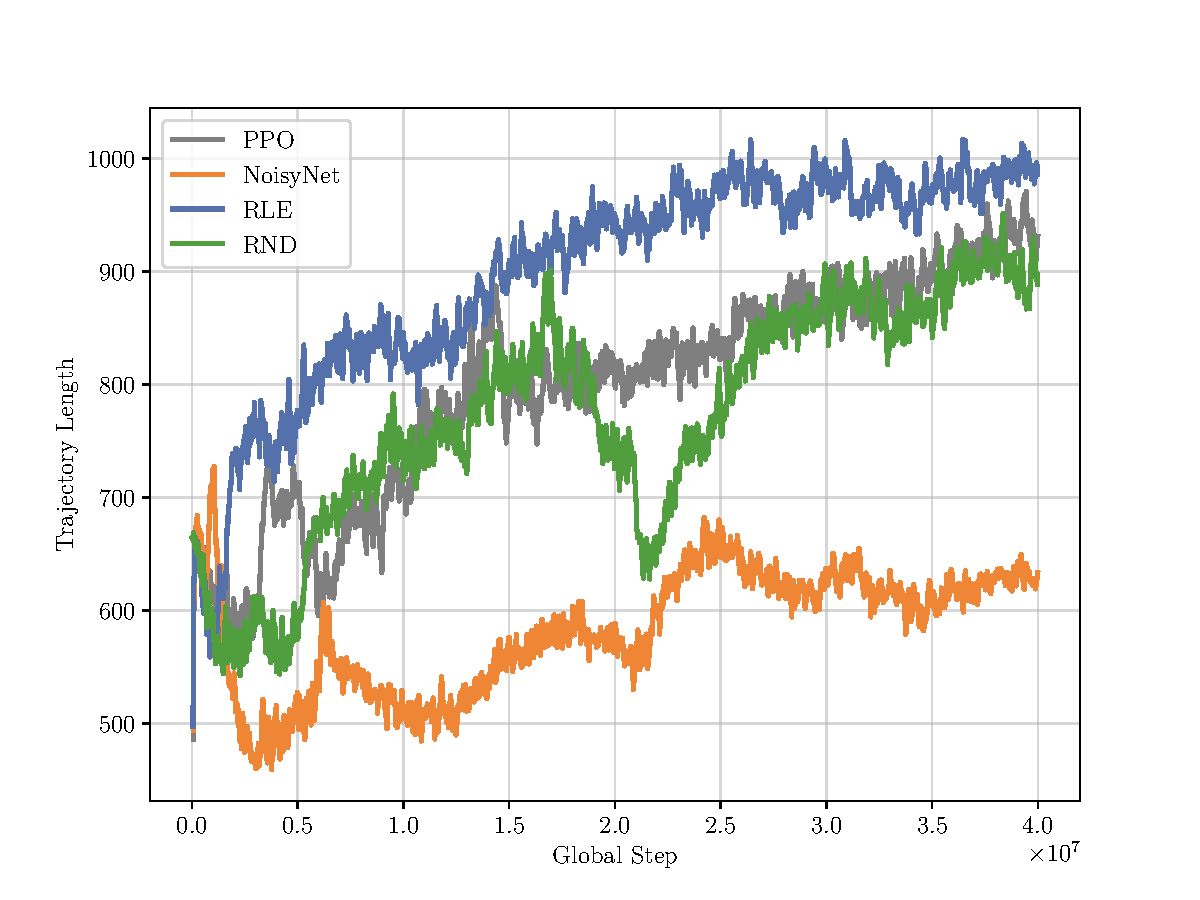
\includegraphics[width=\textwidth]{figures/plot_Alien_TrajectoryLength.pdf}
    \caption{Trajectory Length.}
    \label{fig:alien-trajectorylength}
  \end{subfigure}
  \caption{The \textsc{Alien} game results.}
\end{figure}

\begin{figure}[h!]
  \centering
  \begin{subfigure}[b]{0.45\textwidth}
    \centering
    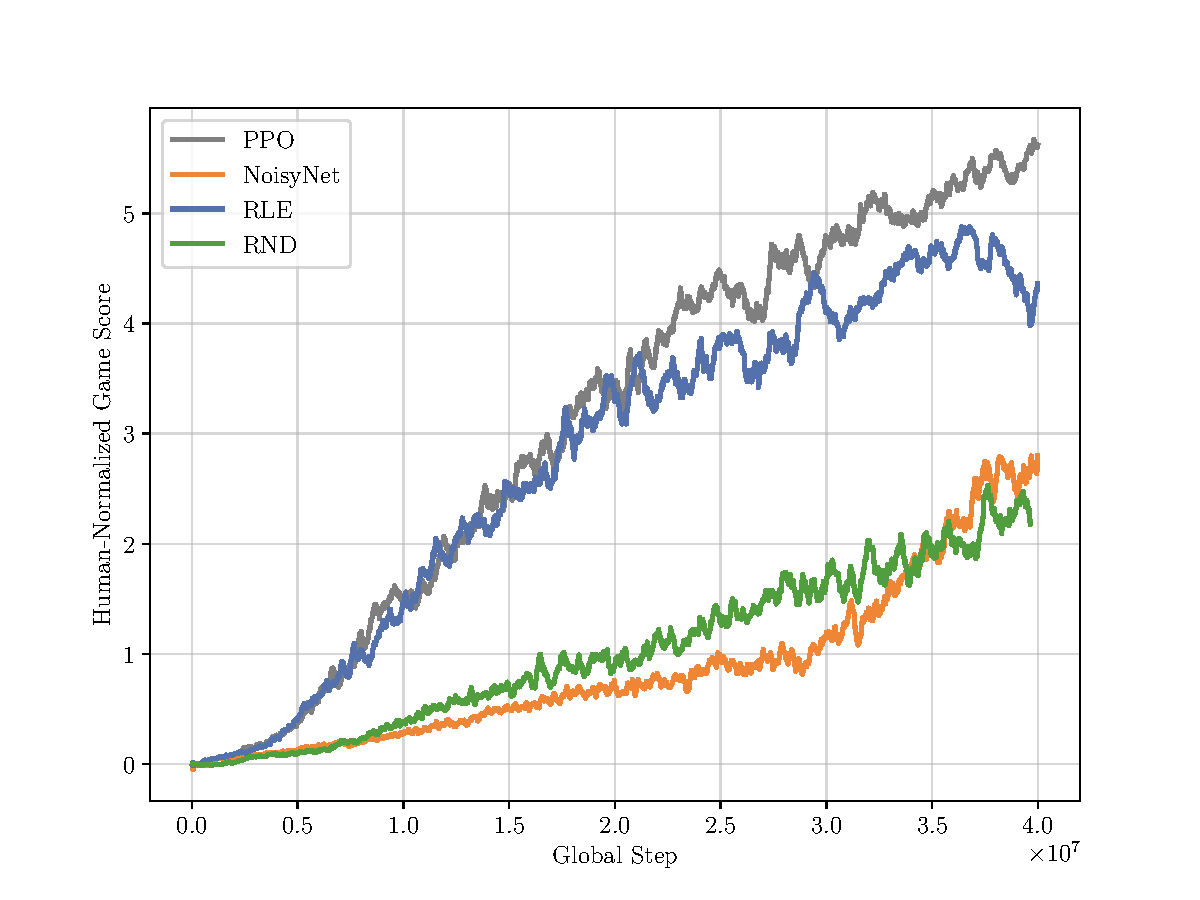
\includegraphics[width=\textwidth]{figures/plot_StarGunner_Score.pdf}
    \caption{Game Score.}
    \label{fig:stargunner-score}
  \end{subfigure}
  \hfill
  \begin{subfigure}[b]{0.45\textwidth}
    \centering
    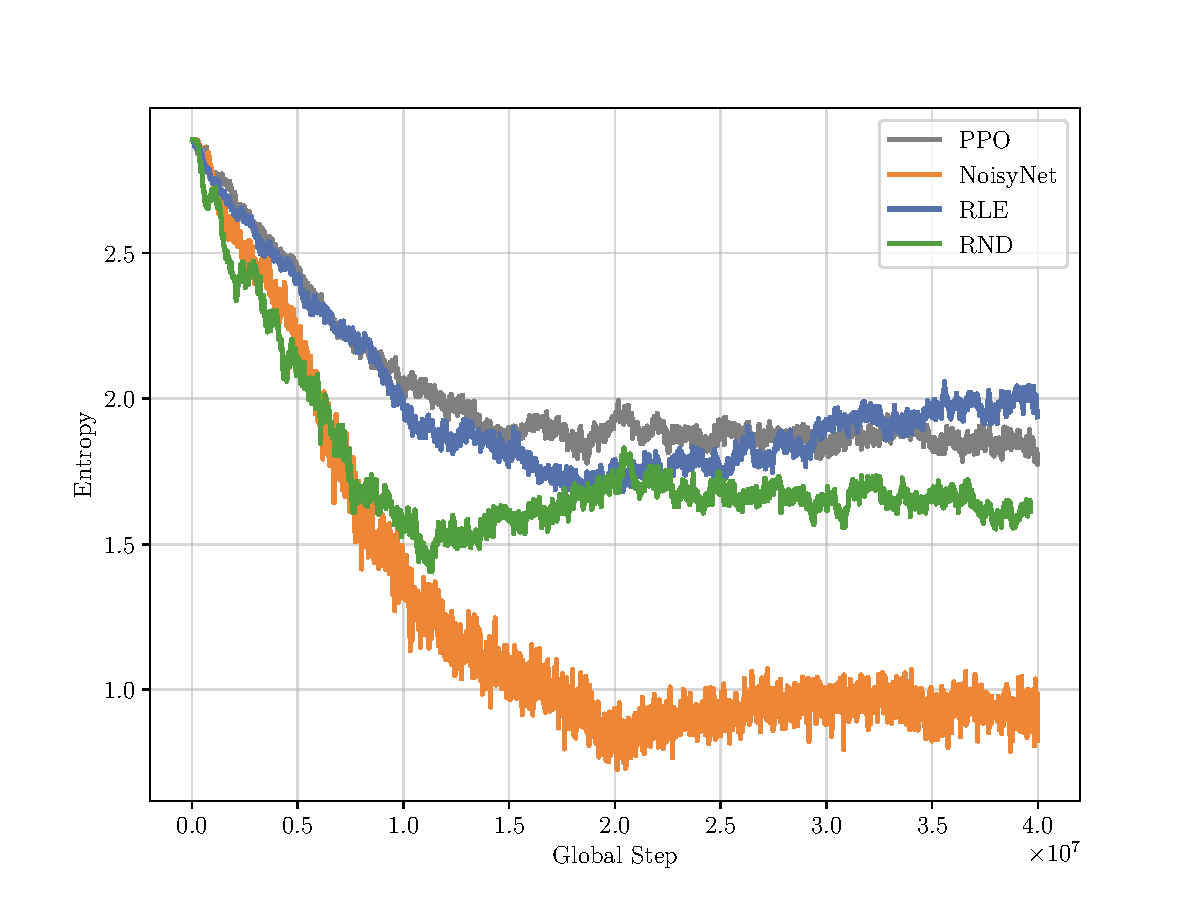
\includegraphics[width=\textwidth]{figures/plot_StarGunner_Entropy.pdf}
    \caption{Entropy.}
    \label{fig:stargunner-entropy}
  \end{subfigure}
  \begin{subfigure}[b]{0.45\textwidth}
    \centering
    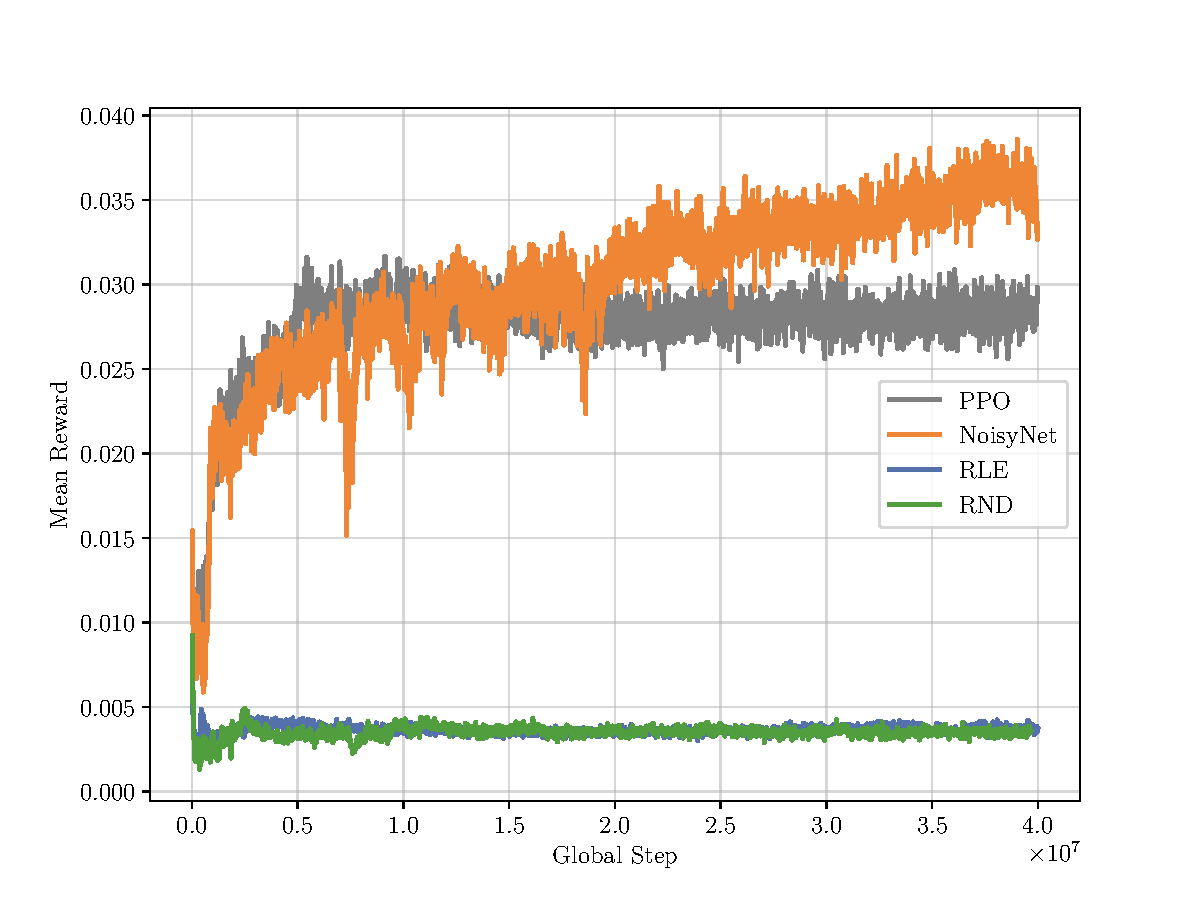
\includegraphics[width=\textwidth]{figures/plot_StarGunner_RewardsMean.pdf}
    \caption{Mean Reward.}
    \label{fig:stargunner-rewards}
  \end{subfigure}
  \hfill
  \begin{subfigure}[b]{0.45\textwidth}
    \centering
    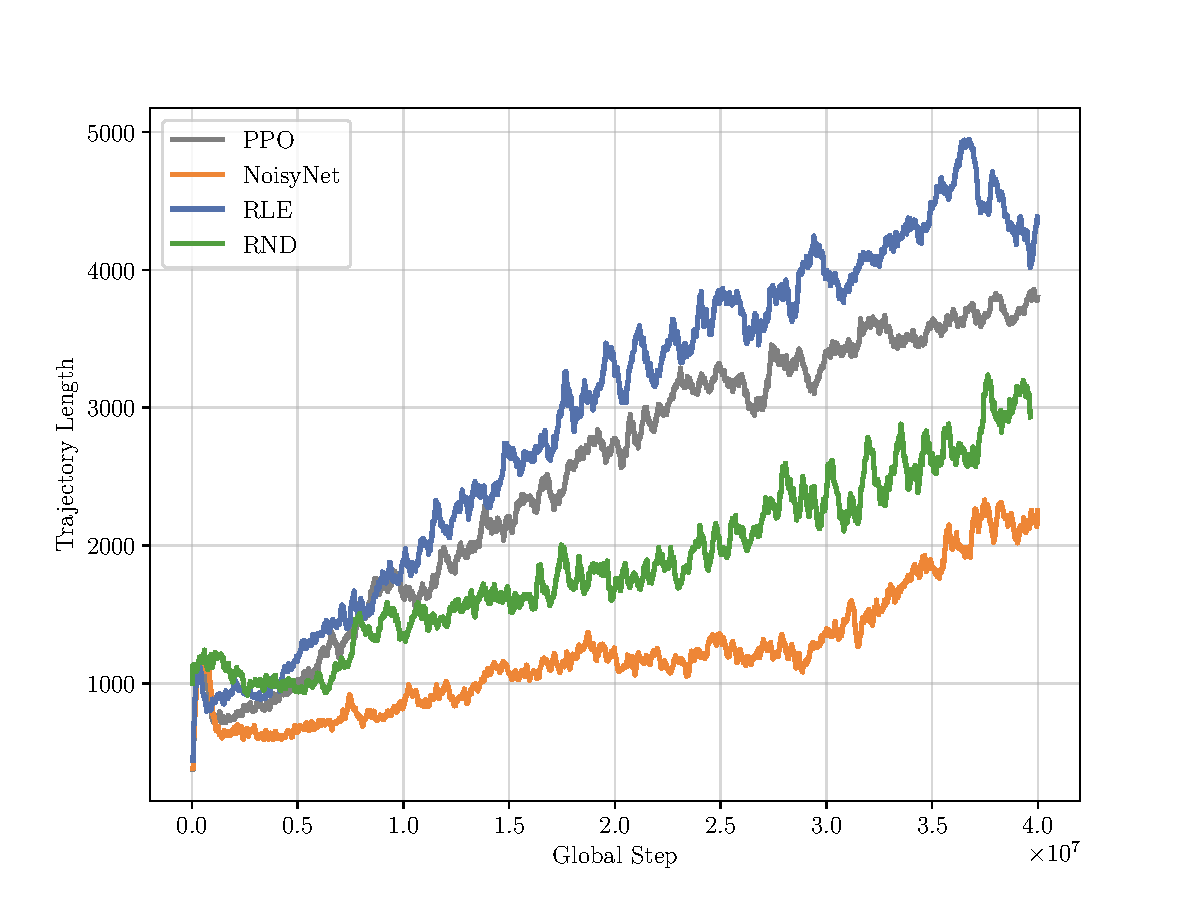
\includegraphics[width=\textwidth]{figures/plot_StarGunner_TrajectoryLength.pdf}
    \caption{Trajectory Length.}
    \label{fig:stargunner-trajectorylength}
  \end{subfigure}
  \caption{The \textsc{StarGunner} game results.}
\end{figure}

\clearpage
\hypertarget{untested-claims}{\section{Untested Claims}}

\noindent The authors made the following claims that, due to time constraints of this project, we were not able to test:

\begin{enumerate}
  \item For the more challenging discrete-action continuous-states\footnote{While the input to the action sampler is a discrete $84\times84\times4$ tensor representing the pixels it perceives, in practice \textsc{Atari} games are considered to be continuous-state environments due to the high-dimensional state space and visual complexity of each frame.} \textsc{Atari} environment, the authors claim that, in the majority of games, \textsc{RLE} achieves a higher IQM of the human-normalized score with a probability of $67\%$, $72\%$ and $71\%$, compared to \textsc{PPO}, \textsc{NoisyNet} and \textsc{RND}, respectively.\footnote{The authors mention that for the \textsc{Montezuma's Revenge} game \textsc{RLE} underperforms likely due to \textsc{RLE} not factoring in bonus-based exploration.}
  \item In the continuous-action continuous-states \textsc{IsaacGym} environment, the authors claim that, with a probability of around $83\%$ for \textsc{PPO}, ca. $66\%$ for \textsc{NoisyNet} and roughly $65\%$ for \textsc{RND}, \textsc{RLE} improves performance in all of their selected \textsc{IsaacGym} tasks.
\end{enumerate}

\noindent Moreover, they performed ablation studies and claimed the following:

\begin{enumerate}
  \item \textsc{RLE} performance compared to \textsc{PPO} is invariant under a change in the dimensionality of the random latent vector.
  \item \textsc{RLE} performance deteriorates if the policy and value networks are not conditioned on the random latent vector.
  \item \textsc{RLE} performance improves slightly if a learning feature network is used in comparison to when the feature network has constant weights when evaluated on the \textsc{Atari} games.
  \item \textsc{RLE} performance is insensitive to the feature extractor architecture.
\end{enumerate}

\clearpage
\hypertarget{appendix-hyperparams}{\section{Hyperparameters}}

\noindent In \textsc{Atari}, we mostly used the same values for the hyperparameters that the authors used. In table \ref{tab:atari-hyperparams} the hyperparameters we modified are summarized. Note that contrary to the authors, due to time constraints we were only able to run every game, of those that we tested, once for each algorithm.

\begin{table}[h!]
  \centering
  \caption{Hyperparameters not stated by \cite{rle-paper} for the \textsc{Atari} experiments.}
  \begin{tabular}{{ll}} 
  \hline
  \textbf{Hyperparameter} & \textbf{Value} \\ \hline
  $\textbf{z}$-Sampling Frequency & $500$\\
  (switch\_steps) & \\
  Norm-\textsc{RLE}-Features & True\\
  Target-KL & None\\
  Anneal Learning Rate & False\\ 
  Target KL Divergence & None\\
  Sticky Action & True\\
  Reward Normalization & True\\
  \end{tabular}
  \label{tab:atari-hyperparams}
\end{table}


\noindent For the \textsc{FourRoom} experiments the hyperparameters stated in \cite{rle-paper} were used. However, \cite{rle-paper} did not provide values for all available hyperparameters. For the missing hyperparameters we used the values in table \ref{tab:gridworld-missing-hyperparameters}, that seemed reasonable to us although we did not spend a lot of time finetuning them.

\begin{table}[h!]
  \centering
  \caption{Hyperparameters not stated by \cite{rle-paper} for the \textsc{FourRoom} experiments.}
  \begin{tabular}{{ll}} 
  \hline
  \textbf{Hyperparameter} & \textbf{Value} \\ \hline
  Extrinsic Reward Coefficient & $1$\\ 
  Observation Normalization Iterations & $1$\\
  Intrinsic Discount Rate & $0.99$ \\ 
  Feature Network Update Rate $\tau$ & $0.005$\\ 
  Anneal Learning Rate & False\\ 
  Target KL Divergence & None\\
  \end{tabular}
  \label{tab:gridworld-missing-hyperparameters}
\end{table}

For the IsaacLab experiments, we assume that the not specified hyperparameters under the \textsc{RLE} experiments section of the paper, were the same as in default \textsc{PPO} implementation which
comprise the following values:
\begin{table}[ht]
\centering
\caption{Hyperparameters not stated by \textcolor{red}{\cite{rle-paper} (I'm assuming you wanted to reference them here)} for \textsc{IsaacLab} experiments.}
\begin{tabular}{{ll}} 
\hline
\textbf{Hyperparameter} & \textbf{Value}\\\hline
Number of Parallel Environments & $4096$\\ 
Rollouts & $8$\\
Learning Epochs & $4$\\
Mini batches & $2$\\
Discount Rate & $0.99$\\
Generalized Advantage Estimation $\lambda$ & $0.95$\\
Gradient Norm Bound & $1.0$\\ 
Used Clipped Value Loss & False \\
Value Loss Scale & $2.0$\\
Timesteps & $5000$\\
\end{tabular}
\label{tab:isaaclab-missing-hyperparameters}
\end{table}
There are two special mentions among these parameters. The number of parallel environments used is $4096$, as it is the default value in the code in the authors repository for 
\textsc{IsaacGym}. In addition, we choose to use a rollout of $8$ as the authors suggested for "AllegroHand" and "ShadowHand" examples for \textsc{CartPole}, which provided higher results than $16$. 
The timestep determination was done by observing a comparable figure with the authors and when the algorithm show a stability around a return. 

\clearpage
\section{Random Latent Exploration}

\noindent The architecture of our \textsc{RLE} implementation can be found in figure \ref{fig:rle-architecture}.

\begin{figure}[h!]
  \centering
  %\includegraphics[width=0.5\textwidth]{tikz/rle-architecture.tex}
  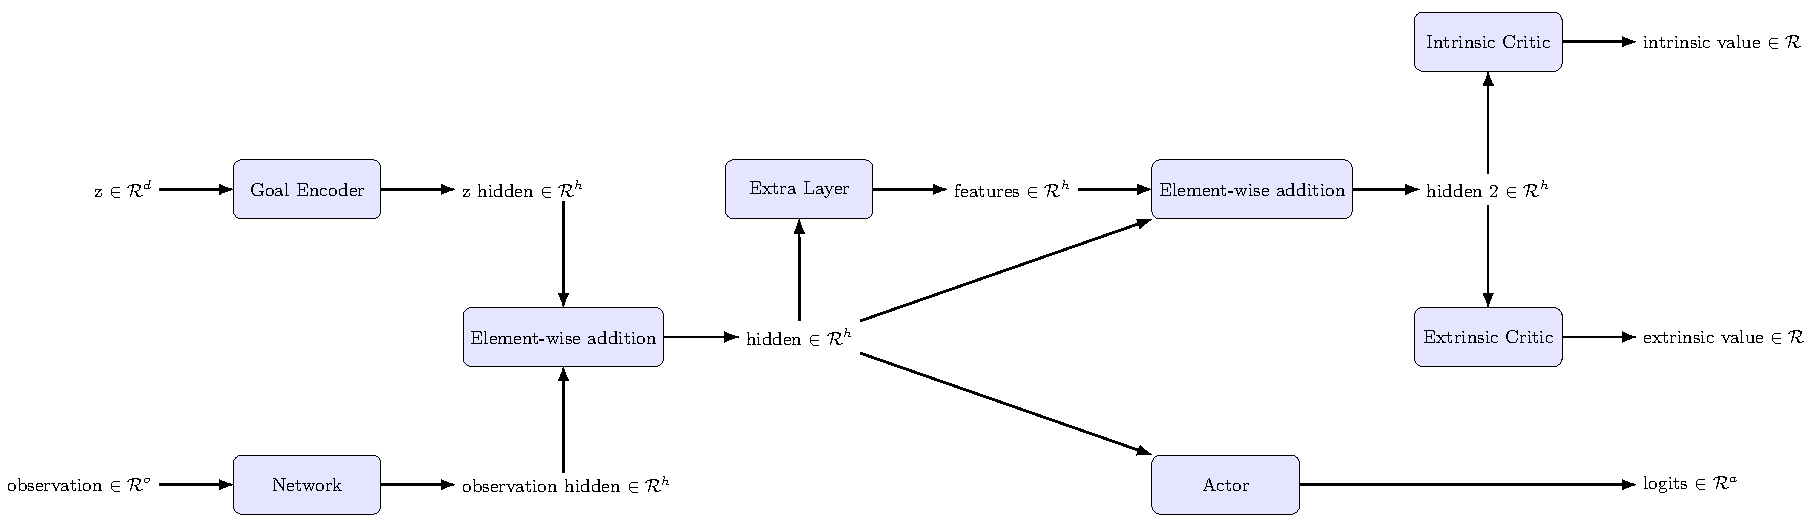
\includegraphics[width=\textwidth]{tikz/rle-architecture-modified.tex}
  \caption{In \textsc{RLE}, the policy and critic networks are conditioned on the latent vector $\textbf{z}$. \cite{rle-paper} split the critic's head in two: one head predicts the extrinsic value and the other head predicts the intrinsic value. In the vector dimension, $o$ represents the dimension of a single observation, $d$ represents the \textsc{RLE} feature dimension, and $a$ is the cardinality of the action space.}
  \label{fig:rle-architecture}
\end{figure}

\noindent For the \textsc{RLE} algorithm, the detailed pseudocode according to \cite{rle-paper} is as follows:

\hypertarget{algo-rle}{
\begin{table}[h!]
  \centering
  \begin{tabular}{rlllll}
    \hline\hline
    \textbf{RLE:} & \multicolumn{5}{l}{Detailed Pseudocode}\\
    \hline
    1: & \multicolumn{5}{l}{\textbf{Input:} Latent distribution $\left(P_{\textbf{z}}\right)$, number of parallel workers $\left(N\right)$, number of steps per update}\\
    & \multicolumn{5}{l}{$\left(T\right)$, number of steps per sampling $\left(S\right)$, and feature network update rate $\left(\tau\right)$.}\\
    2: & \multicolumn{5}{l}{Randomly initialize a feature network $\left(\phi\right)$ with the same backbone architecture as the policy }\\
    & \multicolumn{5}{l}{and value networks.}\\
    3: & \multicolumn{5}{l}{Initialize running mean $\boldsymbol{\mu} = \textbf{0}$ and standard deviation $\boldsymbol{\sigma} = \textbf{1}$ estimates of $\boldsymbol{\phi} \left(s\right)$ over the state}\\
    & \multicolumn{5}{l}{space.}\\
    4: & \multicolumn{5}{l}{Sample an initial latent vector $\textbf{z} \sim P_{\textbf{z}}$ for each parallel worker.}\\
    5: & \multicolumn{5}{l}{\textbf{Repeat (\textsuperscript{1})}}\\
    6: & | & \multicolumn{4}{l}{Sample initial state $s_{0}$.}\\
    7: & | & \multicolumn{4}{l}{\textbf{For} $t = 0, ..., T$ \textbf{do (\textsuperscript{2})}}\\
    8: & | & | & \multicolumn{3}{l}{Take action $a_{t} \sim \boldsymbol{\pi}(. | s_{t}, \textbf{z})$ and transition to $s_{t+1}$.}\\
    9: & | & | & \multicolumn{3}{l}{Compute feature $\textbf{f}(s_{t+1}) = \frac{\boldsymbol{\phi}(s_{t+1}) - \boldsymbol{\mu}}{\boldsymbol{\sigma}}$.}\\
    10: & | & | & \multicolumn{3}{l}{Compute random reward $F(s_{t+1}, \textbf{z}) = \frac{\textbf{f}(s_{t+1})}{\| \textbf{f}(s_{t+1}) \|} \cdot \textbf{z}$.}\\
    11: & | & | & \multicolumn{3}{l}{Receive reward $r_{t} = R(s_{t}, a_{t}) + F(s_{t+1}, \textbf{z})$.}\\
    12: & | & | & \multicolumn{3}{l}{\textbf{For} $i = 0, 1, ..., N-1$ \textbf{do (\textsuperscript{3})}}\\
    13: & | & | & | & \multicolumn{2}{l}{\textbf{If} worker $i$ terminated \textbf{or} $S$ timesteps passed without resampling, \textbf{then (\textsuperscript{4})}}\\
    14: & | & | & | & | & Resample sample $\textbf{z} \sim P_{\textbf{z}}$ for worker $i$.\\
    15: & | & | & | & \multicolumn{2}{l}{\textbf{(\textsuperscript{4})}}\\
    16: & | & | & \multicolumn{3}{l}{\textbf{(\textsuperscript{3})}}\\
    17: & | & \multicolumn{4}{l}{\textbf{(\textsuperscript{2})}}\\
    18: & | & \multicolumn{4}{l}{Update policy network $\boldsymbol{\pi}$ and value network $V_{\boldsymbol{\pi}}$ with the collected trajectory}\\
    & | & \multicolumn{4}{l}{$(\textbf{z}, s_{0}, a_{0}, r_{0}, s_{1}, ..., s_{T})$.}\\
    19: & | & \multicolumn{4}{l}{Update feature network $\boldsymbol{\phi}$ using the value network's parameters $\boldsymbol{\phi} \leftarrow \tau \cdot V^{\boldsymbol{\pi}} + (1 - \tau) \cdot \boldsymbol{\phi}$.}\\
    20: & | & \multicolumn{4}{l}{Update $\boldsymbol{\mu}$ and $\boldsymbol{\sigma}$ using the batch of collected experience.}\\
    21: & \multicolumn{5}{l}{\textbf{(\textsuperscript{1}) until convergence}}\\
    \hline\hline
  \end{tabular}
\end{table}}

\clearpage
\hypertarget{algo-ppo}{\section{Proximal Policy Optimization}}

\noindent The algorithm constituting the foundation of \textsc{RLE} is Proximal Policy Iteration (\textsc{PPO}), described in \cite{ppo-paper}, which can itself be run to solve RL problems. It is an on-line policy gradient method where after running the policy $\boldsymbol{\pi}_{\theta_{\text{old}}}$ in parallel with $N$ actors for $T << E$ timesteps, where $E$ is the length of an episode, we compute the advantage estimator as proposed by \cite{generalized-advantage-estimation-paper} for each time index $t \in [0, T]$:

\begin{equation}
  \hat{A}_{t} = \delta_{t} + \left(\gamma \lambda\right) \delta_{t+1} + ... + \left(\gamma \lambda\right)^{T-t+1} \delta_{T - 1}
  \label{eq:ppo-advantage-estimator}
\end{equation}

\noindent where we have $\delta_{t} = r_{t} + \gamma V(s_{t+1}) - V(s_{t})$. Here, $\lambda$ is the Generalized Advantage Estimation (GAE) parameter and $V(s)$ is a learned state-value function. Afterwards, for each $t$ the surrogate objective is computed and the parameters $\theta$ are optimized e.g. with minibatch SGD or Adam (note that we optimize by maximizing the objective). This surrogate objective takes the form:

\begin{equation}
  L_{t}^{\text{CLIP} + \text{VF} + \text{S}}(\theta) = \hat{\mathbb{E}}_{t} \left[L_{t}^{\text{CLIP}}(\theta) - c_{1} L_{t}^{\text{VF}}(\theta) + c_{2} S[\boldsymbol{\pi}_{\theta}](s_{t})\right]
  \label{eq:ppo-objective-function}
\end{equation}

\noindent In \eqref{eq:ppo-objective-function}, we have the VF coefficient $c_{1}$ and the entropy coefficient $c_{2}$, together with the (optional, to enhance exploration) entropy bonus $S[\boldsymbol{\pi}_{\theta}](s_{t})$, which is calculated as the sum of $- p \log{p}$ over each of the action-probabilities $p$ resulting from the policy distribution $\boldsymbol{\pi}_{\theta}$ for a state $s_{t}$, and the objectives:

\begin{align}
  \label{eq:ppo-clip-objective} L_{t}^{\text{CLIP}}(\theta) &= \hat{\mathbb{E}}_{t}\left[\min\left(r_{t}(\theta) \hat{A}_{t}, \text{clip}\left(r_{t}(\theta), 1 - \epsilon, 1 + \epsilon\right) \hat{A}_{t}\right)\right]\\
  \label{eq:ppo-vf-objective} L_{t}^{\text{VF}}(\theta) &= \left(V_{\theta}(s_{t}) - V_{t}^{\text{targ}}\right)^{2}
\end{align}

\noindent In \eqref{eq:ppo-clip-objective} we denote the probability ratio as $r_{t}(\theta) = \frac{\pi_{\theta}\left(a_{t}|s_{t}\right)}{\pi_{\theta_{\text{old}}}(a_{t}|s_{t})}$, where $\pi_{\theta_{\text{old}}}$ is the policy before the update, and the clipping function is:

\begin{equation}
  \text{clip}\left(r_{t}(\theta), 1 - \epsilon, 1 + \epsilon\right) = \begin{cases}
    1 - \epsilon, &r_{t}(\theta) < 1 - \epsilon\\
    r_{t}(\theta), &1 - \epsilon \leq r_{t}(\theta) \leq 1 + \epsilon\\
    1 + \epsilon, &r_{t}(\theta) > 1 + \epsilon
  \end{cases}
  \label{eq:clipping-function}
\end{equation}

\noindent Moreover in \eqref{eq:ppo-vf-objective}, $V_{t}^{\text{targ}}$ represents some target state-value function that is to be obtained. Note that there exist also other objective functions mentioned in \cite{ppo-paper} that can substitute $L_{t}^{\text{CLIP}}(\theta)$ in \eqref{eq:ppo-objective-function}. In \eqref{eq:clipping-function}, we make use of a hyperparameter $\epsilon \in [0, 1]$ and in combination with the minimizer from \eqref{eq:ppo-clip-objective} we can prevent a single policy update to accidentally ruin the policy forever by sending the algorithm to a gradient region with a worse local extremum.

\noindent For the \textsc{PPO} algorithm, the detailed pseudocode according to \cite{ppo-paper} is as follows:

\begin{table}[h!]
  \centering
  \begin{tabular}{rlll}
    \hline\hline
    \textbf{PPO:} & \multicolumn{3}{l}{Detailed Pseudocode, Actor-Critic Setup}\\
    \hline
    1: & \multicolumn{3}{l}{\textbf{Input:} Number of iterations $\left(I\right)$, number of actors $\left(N\right)$, number of timesteps per iteration}\\
    & \multicolumn{3}{l}{$\left(T\right)$, number of epochs $(K)$, minibatch size $(M \leq NT)$, learned state-value function implicitly}\\
    & \multicolumn{3}{l}{in the advantage estimator $(V(s))$, target value $(V_{t}^{\text{targ}})$ implicitly in the objective $L$.}\\
    2: & \multicolumn{3}{l}{\textbf{For} $i = 1, ..., I$ \textbf{do (\textsuperscript{1})}}\\
    3: & | & \multicolumn{2}{l}{\textbf{For} $n = 1, ..., N$ \textbf{do (\textsuperscript{2})}}\\
    4: & | & | & Run policy $\boldsymbol{\pi}_{\theta_{\text{old}}}$ in environment for $T$ timesteps.\\
    5: & | & | & Compute advantage estimates $\hat{A}_{1}, ..., \hat{A}_{T}$.\\
    6: & | & \multicolumn{2}{l}{\textbf{(\textsuperscript{2})}}\\
    7: & | & \multicolumn{2}{l}{Optimize objective $L$ w.r.t. $\theta$, for given $K$ and $M$, using e.g. minibatch SGD or Adam.}\\
    8: & | & \multicolumn{2}{l}{Update parameters $\theta_{\text{old}} \leftarrow \theta$.}\\
    9: & \multicolumn{3}{l}{\textbf{(\textsuperscript{1})}}\\
    \hline\hline
  \end{tabular}
\end{table}

\clearpage
\hypertarget{algo-noisynet}{\section{NoisyNet}}

\noindent The central idea in a \textsc{NoisyNet} architecture brought forward by \cite{noisynet-paper} is to introduce random noise into the weights learned by the network ($p$ inputs, $q$ outputs), i.e. if we have a neural network whose output can be parametrized by a vector of weights $\boldsymbol{\theta}$ as $\textbf{y} = f_{\boldsymbol{\theta}}(\textbf{x}) = \textbf{w} \cdot \textbf{x} + \textbf{b}$, then we can learn the set of parameter vectors $\zeta = (\boldsymbol{\mu}, \boldsymbol{\Sigma})$ to compute $\textbf{w} = (\boldsymbol{\mu}^{w} + \boldsymbol{\sigma}^{w} \odot \boldsymbol{\varepsilon}^{w})$ and $\textbf{b} = (\boldsymbol{\mu}^{b} + \boldsymbol{\sigma}^{b} \odot \boldsymbol{\varepsilon}^{b})$ with the following dimensionalities: $\boldsymbol{\mu}^{w}$, $\boldsymbol{\sigma}^{w}$, $\boldsymbol{\varepsilon}^{w} \in \mathbb{R}^{q \times p}$ implying $\textbf{w} \in \mathbb{R}^{q \times p}$, and $\boldsymbol{\mu}^{b}$, $\boldsymbol{\sigma}^{b}$, $\boldsymbol{\varepsilon}^{b} \in \mathbb{R}^{q}$ resulting in $\textbf{b} \in \mathbb{R}^{q}$. Note that $\textbf{x} \in \mathbb{R}^{p}$, $\textbf{y} \in \mathbb{R}^{q}$ and $\odot$ denotes element-wise multiplication.

\noindent We optimize the loss $\bar{L}(\zeta) = \mathbb{E}_{\varepsilon}[L(\boldsymbol{\theta})]$, i.e. the expectation of the loss $L(\boldsymbol{\theta})$ over the noise $\varepsilon$ which has a mean of zero and fixed statistics, using gradient descent on the parameters $\zeta$. The noise can be sampled either independently or in a factorized way from a Gaussian. The former method samples the noise $\varepsilon^{w}_{i,j} \in \boldsymbol{\varepsilon}^{w}$ and $\varepsilon^{b}_{j} \in \boldsymbol{\varepsilon}^{b}$ for every input to the network leading to a total of $pq + q$ random samples. Factorized sampling on the other hand greatly reduces computational complexity by factorizing $\varepsilon^{w}_{i,j} = f(\varepsilon_{i}) f(\varepsilon_{j})$ and then $\varepsilon^{b}_{j} = f(\varepsilon_{j})$ thereby lowering the number of required random samples to $p + q$, where $f: \mathbb{R} \rightarrow \mathbb{R}$. In \cite{noisynet-paper} the function $f(x) = \sign(x) \sqrt{|x|}$ is used. After sampling the noise, in theory we compute the gradients $\nabla\bar{L}(\zeta) = \nabla\mathbb{E}_{\varepsilon}[L(\boldsymbol{\theta})] = \mathbb{E}_{\varepsilon}[\nabla_{\boldsymbol{\mu}, \boldsymbol{\Sigma}}L(\boldsymbol{\mu} + \boldsymbol{\Sigma} \odot \boldsymbol{\varepsilon})]$, whereas in practice we approximate $\nabla\bar{L}(\zeta) \approx \nabla_{\boldsymbol{\mu}, \boldsymbol{\Sigma}}L(\boldsymbol{\mu} + \boldsymbol{\Sigma} \odot \boldsymbol{\varepsilon})$ with the Monte Carlo method.

\noindent In the code of \cite{rle-paper}, a \textsc{NoisyNet} is used in conjunction with the A3C-algorithm, in particular the loss is computed from the action-value function is estimated using:

\begin{equation}
  \hat{Q}_{i} = \sum_{j=i}^{k-1} \gamma^{j-i} r_{t+j} + \gamma^{k-i} V(x_{t+k} | \zeta, \varepsilon_{i})
\end{equation}

Moreover, for factorized networks, we initialize $\mu_{i,j} \sim \mathcal{U}\left[-\frac{1}{\sqrt{p}}, +\frac{1}{\sqrt{p}}\right]$ and $\sigma_{i,j} = \frac{\sigma_{0}}{\sqrt{p}}$ with $p$ being the number of inputs to the corresponding linear layer, $\mathcal{U}$ is a uniform distribution over the specified interval, and $\sigma_{0}$ is a hyperparameter.

\noindent For the \textsc{NoisyNet} + A3C algorithm, the detailed pseudocode according to \cite{noisynet-paper} is as follows:

\begin{table}[H]
  \centering
  \begin{tabular}{rlll}
    \hline\hline
    \textbf{NoisyNet:} & \multicolumn{3}{l}{Detailed Pseudocode, for each actor-learner thread}\\
    \hline
    1: & \multicolumn{3}{l}{\textbf{Input:} Global shared parameters $(\zeta_{\pi}, \zeta_{V})$, global shared counter $(T)$, and maximal}\\
    & \multicolumn{3}{l}{time $(T_{\text{max}})$.}\\
    2: & \multicolumn{3}{l}{\textbf{Input (each thread):} Thread-specific parameters $(\zeta_{\pi}', \zeta_{V}')$, set of random variables $(\varepsilon)$,}\\
    & \multicolumn{3}{l}{thread-specific counter $(t)$, and roll-out size $(t_{\text{max}})$.}\\
    3: & \multicolumn{3}{l}{\textbf{Output:} Policy $\pi(\cdot|\zeta_{\pi}, \varepsilon)$ and value function $V(\cdot|\zeta_{V},\varepsilon)$.}\\
    4: & \multicolumn{3}{l}{$t \leftarrow 1$}\\
    5: & \multicolumn{3}{l}{\textbf{Repeat (\textsuperscript{1})}}\\
    6: & | & \multicolumn{2}{l}{Reset cumulative gradients: $d\zeta_{\pi} \leftarrow 0, d\zeta_{V} \leftarrow 0$.}\\
    7: & | & \multicolumn{2}{l}{Synchronize thread-specific parameters: $\zeta_{\pi}' \leftarrow \zeta_{\pi}, \zeta_{V}' \leftarrow \zeta_{V}$.}\\
    8: & | & \multicolumn{2}{l}{Set counter $c \leftarrow 0$.}\\
    9: & | & \multicolumn{2}{l}{Get state $x_{t}$ from environment.}\\
    10: & | & \multicolumn{2}{l}{Sample noise $\xi \sim \varepsilon$.}\\
    11: & | & \multicolumn{2}{l}{Create lists for rewards $r \leftarrow [ ]$, actions $a \leftarrow [ ]$ and states $x \leftarrow [ ]$.}\\
    12: & | & \multicolumn{2}{l}{\textbf{Repeat (\textsuperscript{2})}}\\
    13: & | & | & Choose action $a_{t} \leftarrow \pi(\cdot|x_{t}, \zeta_{pi}', \zeta_{V}')$.\\
    14: & | & | & $a[-1] \leftarrow a_{t}$\\
    15: & | & | & Obtain reward $r_{t}$ and new state $x_{t+1}$.\\
    16: & | & | & $r[-1] \leftarrow r_{t}$, $x[-1] \leftarrow x_{t}$, $t \leftarrow t + 1$, $T \leftarrow T + 1$, $c \leftarrow c + 1$\\
    17: & | & \multicolumn{2}{l}{\textbf{(\textsuperscript{2}) until} $x_{t}$ \textbf{is terminal or} $c > t_{\text{max}}$}\\
    18: & | & \multicolumn{2}{l}{\textbf{If} $x_{t}$ is terminal, \textbf{then (\textsuperscript{3})}}\\
    19: & | & | & $Q \leftarrow 0$\\
    20: & | & \multicolumn{2}{l}{\textbf{else}}\\
    21: & | & | & $Q \leftarrow V\left(x_{t}|\zeta_{V}', \xi\right)$\\
    22: & | & \multicolumn{2}{l}{\textbf{(\textsuperscript{3})}}\\
    23: & | & \multicolumn{2}{l}{\textbf{For} $i = c - 1, ..., 0$ \textbf{do (\textsuperscript{4})}}\\
    24: & | & | & $Q \leftarrow r\left[i\right] + \gamma Q$\\
    25: & | & | & $d\zeta_{\pi} \leftarrow d\zeta_{\pi} \nabla_{\zeta_{\pi}'} \log{(\pi(a[i]|x[i], \zeta_{\pi}', \xi)) [Q - V(x[i]|\zeta_{V}', \xi)]}$\\
    26: & | & | & $d\zeta_{V} \leftarrow d\zeta_{V} \nabla_{\zeta_{V}'} \left[Q - V\left(x[i]|\zeta_{V}', \xi\right)\right]^{2}$\\
    27: & | & \multicolumn{2}{l}{\textbf{(\textsuperscript{4})}}\\
    28: & | & \multicolumn{2}{l}{Update asynchronously parameter $\zeta_{\pi} \leftarrow \zeta_{\pi} + \alpha_{\pi}d\zeta_{\pi}$.}\\
    29: & | & \multicolumn{2}{l}{Update asynchronously parameter $\zeta_{V} \leftarrow \zeta_{V} - \alpha_{V}d\zeta_{V}$.}\\
    30: & \multicolumn{3}{l}{\textbf{(\textsuperscript{1}) until} $T > T_{\text{max}}$}\\
    \hline\hline
  \end{tabular}
\end{table}

\clearpage
\hypertarget{algo-rnd}{\section{Random Network Distillation}}

In Random Network Distillation, as described by \cite{rnd-paper}, we compose the reward which the agent obtains as $r_{t} = e_{t} + i_{t}$ where $e_{t}$ represents a sparse extrinsic (environment's) reward and $i_{t}$ is the intrinsic reward for transitioning, i.e. the exploration bonus emanating from the transition at time step $t$. The latter measures the novelty of a state and should yield a higher value, the less frequently a state has been visited so far. In case of a finite state space we can use $i_{t} = \frac{1}{n_{t}}$ or $i_{t} = \frac{1}{\sqrt{s}}$ where $n_{t}(s)$ denotes the number of times state $s$ has been visited until time step $t$. However, there exist alternatives, e.g. we could use state density based approaches to calculate an exploration bonus, which are described in the paper mentioned above. Moreover, they specify that in the paper the intrinsic reward is the prediction error of a randomly generated problem $i_{t} = \|\hat{f}(x|\theta) - f(x)\|^{2}$ involving a target network $f: \mathcal{O} \rightarrow \mathbb{R}^{k}$ (fixed and randomly initialized, maps an observation $\mathcal{O}$ to an embedding $\mathbb{R}^{k}$) to sample the problem as well as a predictor network $\hat{f}: \mathcal{O} \rightarrow \mathbb{R}^{k}$ which was trained on the agent's data by gradient descent to optimize $i_{t}$ w.r.t. parameters $\theta_{\hat{f}}$.

\noindent Since the overall return can be composed as a sum of returns $R = R_{E} + R_{I}$ we can train two heads $V_{E}$ and $V_{I}$ to estimate the value function $V = V_{E} + V_{I}$ and in extension the advantages. In the end, a policy is trained with standard \textsc{PPO} using the advantage estimators. Note that the intrinsic rewards have to be normalized in order to be useful because otherwise we could not guarantee that they are on a consistent scale, which is done by dividing $i_{t}$ by a running estimate of the standard deviations of the intrinsic return. Furthermore, the observation also has to be normalized as $x \leftarrow \text{clip}(\frac{x - \mu}{\sigma}, -5, 5)$. The normalization parameters can be initialized by letting a random agent briefly move in the environment before beginning the optimization.

\noindent The detailed pseudocode according to \cite{rnd-paper} is as follows:

\begin{table}[H]
  \centering
  \begin{tabular}{rlll}
    \hline\hline
    \textbf{RND:} & \multicolumn{3}{l}{Detailed Pseudocode}\\
    \hline
    1: & \multicolumn{3}{l}{\textbf{Input:} Number of rollouts $(N)$, Number of optimization steps $(N_{\text{opt}})$, and length of initial}\\
    & \multicolumn{3}{l}{steps for initializing observation normalization $(M)$.}\\
    2: & \multicolumn{3}{l}{$t \leftarrow 0$}\\
    3: & \multicolumn{3}{l}{Sample state $s_{0} \sim p_{0}(s_{0})$.}\\
    4: & \multicolumn{3}{l}{\textbf{For} $m = 1, ..., M$ \textbf{do (\textsuperscript{1})}}\\
    5: & | & \multicolumn{2}{l}{Sample action $a_{t} \sim \mathcal{U}(a_{t})$.}\\
    6: & | & \multicolumn{2}{l}{Sample state $s_{t+1} \sim p(s_{t+1}|s_{t}, a_{t})$.}\\
    7: & | & \multicolumn{2}{l}{Update observation normalization parameters using $s_{t+1}$.}\\
    8: & | & \multicolumn{2}{l}{$t \leftarrow t + 1$}\\
    9: & \multicolumn{3}{l}{\textbf{(\textsuperscript{1})}}\\
    10: & \multicolumn{3}{l}{\textbf{For} $i = 1, ..., N$ \textbf{do (\textsuperscript{2})}}\\
    11: & | & \multicolumn{2}{l}{\textbf{For} $j = 1, ..., K$ \textbf{do (\textsuperscript{3})}}\\
    12: & | & | & Sample action $a_{t} \sim \pi(a_{t}|s_{t})$.\\
    13: & | & | & Sample state $s_{t+1}, e_{t} \sim p(s_{t+1}, e_{t}|s_{t}, a_{t})$.\\
    14: & | & | & Calculate intrinsic reward $i_{t} = \|\hat{f}(s_{t+1}) - f(s_{t+1})\|^{2}$.\\
    15: & | & | & Add $s_{t}, s_{t+1}, a_{t}, e_{t}, i_{t}$ to optimization batch $B_{i}$.\\
    16: & | & | & Update running estimate of reward standard deviation using $i_{t}$.\\
    17: & | & | & $t \leftarrow t + 1$\\
    18: & | & \multicolumn{2}{l}{\textbf{(\textsuperscript{3})}}\\
    19: & | & \multicolumn{2}{l}{Normalize the intrinsic rewards contained in $B_{i}$.}\\
    20: & | & \multicolumn{2}{l}{Calculate returns $R_{I,i}$ and advantages $A_{I,i}$ for intrinsic reward.}\\
    21: & | & \multicolumn{2}{l}{Calculate returns $R_{E,i}$ and advantages $A_{E,i}$ for extrinsic reward.}\\
    22: & | & \multicolumn{2}{l}{Calculate combined advantages $A_{i} = A_{I,i} + A_{E,i}$.}\\
    23: & | & \multicolumn{2}{l}{Update observation normalization parameters using $B_{i}$.}\\
    24: & | & \multicolumn{2}{l}{\textbf{For} $j = 1, ..., N_{\text{opt}}$ \textbf{do (\textsuperscript{4})}}\\
    25: & | & | & Optimize $\theta_{\pi}$ w.r.t. \textsc{PPO} loss on batch $B_{i}, R_{i}, A_{i}$ using Adam.\\
    26: & | & | & Optimize $\theta_{\hat{f}}$ w.r.t. distillation loss on $B_{i}$ using Adam.\\
    27: & | & \multicolumn{2}{l}{\textbf{(\textsuperscript{4})}}\\
    28: & \multicolumn{3}{l}{\textbf{(\textsuperscript{2})}}\\
    \hline\hline
  \end{tabular}
\end{table}

\clearpage
\hypertarget{na-vmf}{\section{Neural-adaptive VMF}}

Even more interesting was the construction of the loss that can guide the training of the networks. We first have an \textsc{alignment} term:

\begin{equation}
    \mathcal{L}_{align} = - \sum_{t=1}^{T} \langle \boldsymbol{\mu}_{t-1}, \textbf{z}_{t-1} \rangle \cdot r_{t}
\end{equation}

Such that when sampled $z$ from a VMF with $\mu$ as direction produced high return $r$ that will be seen in the next step, then most we want $\mu$ to be like $z$, aligning $\mu$ with the highest rewarding $z$.

The second term of the loss is the differential entropy of VMF:

\begin{equation}
    H(\text{vMF}) = -\log(C_d(\kappa)) - \kappa A_d(\kappa)
\end{equation}

where:
\begin{equation}
    C_d(\kappa) = \frac{\kappa^{d/2-1}}{(2\pi)^{d/2}I_{d/2-1}(\kappa)}
\end{equation}

\begin{equation}
    A_d(\kappa) = \frac{I_{d/2}(\kappa)}{I_{d/2-1}(\kappa)}
\end{equation}

Taking the logarithm of $C_d(\kappa)$:
\begin{equation}
    \log(C_d(\kappa)) = (d/2-1)\log(\kappa) - \frac{d}{2}\log(2\pi) - \log(I_{d/2-1}(\kappa))
\end{equation}

Therefore, the complete entropy expression is:
\begin{equation}
  \mathcal{L}_{entropy} = -\left[(d/2-1)\log(\kappa) - \frac{d}{2}\log(2\pi) - \log(I_{d/2-1}(\kappa))\right] - \kappa\frac{I_{d/2}(\kappa)}{I_{d/2-1}(\kappa)}
\end{equation}

This term pushes the model for exploration (lower $\kappa$) with two weighting parameters, one based on progress such that the term decays while training progresses and another based on stagnation, such that if the recent returns show little variation compared to the overall returns (over a short window), indicating stagnation, the function increases the exploration boost.

The third term is the \textsc{reward} loss -- Huber loss:

\begin{equation}
    \mathcal{L}_{huber} = \sum_{t=1}^{T} \begin{cases} 
    \frac{1}{2} \left( r_{t} - \hat{r}_{t} \right)^{2}, & \text{if } \left| r_{t} - \hat{r}_{t} \right| < \delta \\
    \delta \left( \left| r_{t} - \hat{r}_{t} \right| - \frac{1}{2} \delta \right), & \text{otherwise}
    \end{cases}
\end{equation}

We use the Huber loss since reward can be sparse and since what we finally want to teach the model is to differentiate what are good states to be in compared to others then, we can soften the effect of these outliers such that the small errors goes under the quadratic loss whereas the outliers receive a linear loss, reducing their impact on the final loss. 

We also need to teach the model how to form a confidence around a certain $\mu$. The $\kappa$-loss is constructed by first estimating a good target $\kappa$, which can be done by setting a maximum and minimum $\kappa$ bound. Visualizing the VMF distribution helps to notice that a $k \in [0,40]$ is a good range, allowing still even reaching the maximum to sample values at a certain range of distance from $\mu$, allowing for exploration.

\begin{equation}
    \kappa_{target} = \kappa_{min} + (\kappa_{max} - \kappa_{min}) \cdot \text{returns}_{scaled}
\end{equation}

The scaled returns are passed through a sigmoid, which means that kappa final value will be proportional to the range between max and min bounds of kappa where that proportion is determined by the returns produced by the corresponding $z$. Then, this target will be the input of the Huber loss for kappa. Although, it can be use an MSE loss too. 

Finally, there is an optional term, \textsc{KL-divergence} term. The idea of this term is to naturally provide a consistent exploration. The authors in the paper offered to set resampling of $z$ after certain steps, but it could be controlled naturally by restricting the distributions change in this case. However, this term is not exploited in \textsc{Alien} due to the time constrain.\footnote{The respective method is implemented in the code.}

Is important to notice that we develop each method with PyTorch, even considering that there is no Bessel function of higher order than one in the library. 
However, there is a beautiful property of Bessel functions that allow to write the higher order as a function of the previous two.\footnote{\url{https://proofwiki.org/wiki/Recurrence_Formula_for_Bessel_Function_of_the_First_Kind}} Since the first two  orders of the first kind Bessel functions are implemented, then we had all the ingredients to make a perfect differentiable \textsc{entropy} and \textsc{KL-divergence} term which will be necessary for BPTT. In addition, could be interesting to test what would happen if we keep the cell (long term) memory of the LSTM between episodes of the same parallel environment.

\begin{figure}[H]
  \centering
  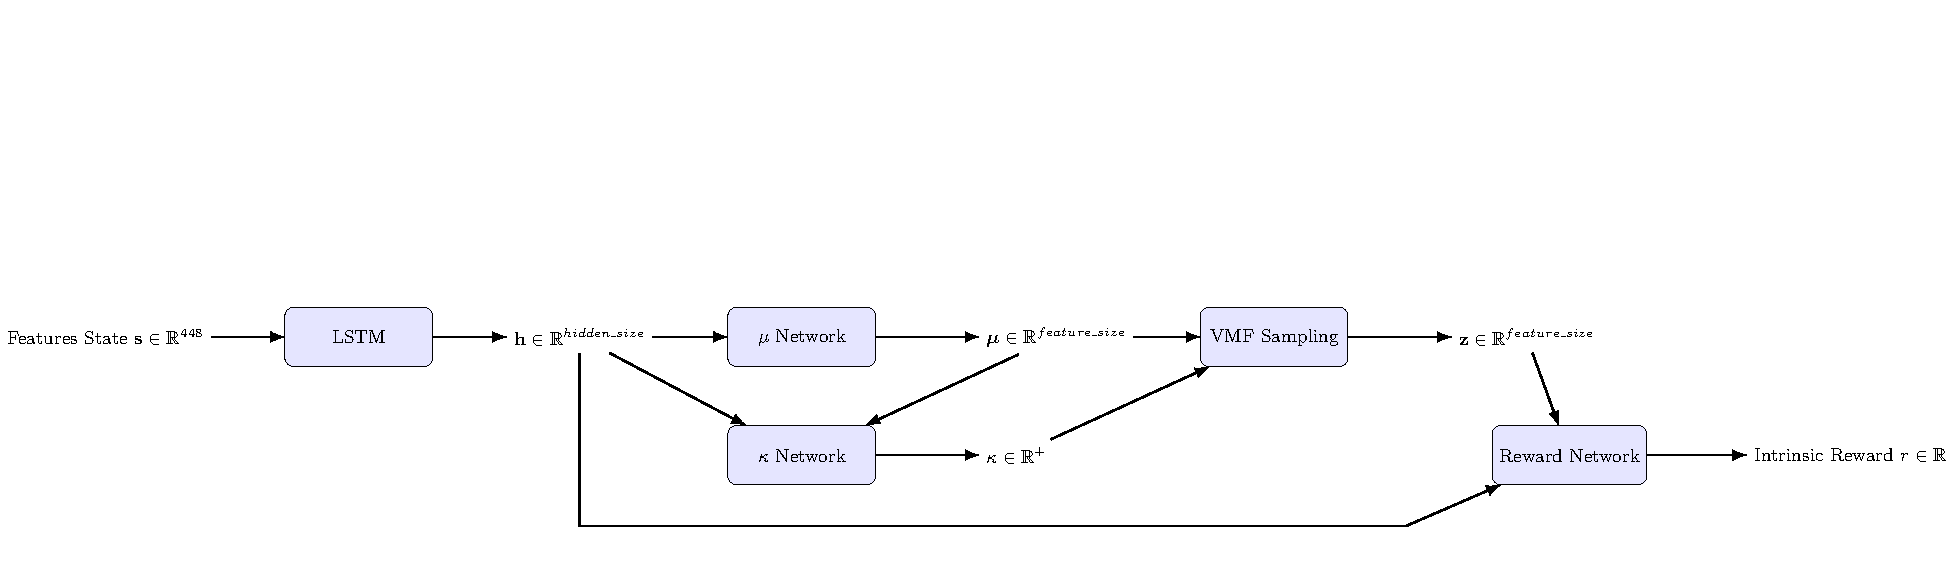
\includegraphics[width=\textwidth]{tikz/neural-adaptive-vmf.tex}
  \caption{Neural-adaptive VMF architecture.}
  \label{fig:neural-adaptive-vmf}
\end{figure}

\begin{table}[h!]
  \centering
  \caption{Results of the \textsc{Atari} experiments with Adaptive VMF}
  \begin{subtable}[h]{0.48\textwidth}
      \centering
      \begin{tabular}{{llll}} 
        \hline
        \textbf{Algorithm} & & Game Score & Human-Norm.\\
        \hline
        QVMF & & $2184$ & $0.285$\\
        NAVMF & & $2109$ & $0.273$\\ 
        \textsc{RLE} & & $1626$ & $0.203$\\ 
        \textsc{PPO} & & $1384$ & $0.168$
    \end{tabular}
    \caption{\textsc{Alien-V5}}
    \label{tab:alien-score-vmf}
  \end{subtable}
  \label{tab:atari-results-vmf}
  \vspace{-18pt}
\end{table}

\begin{figure}[H]
  \centering
  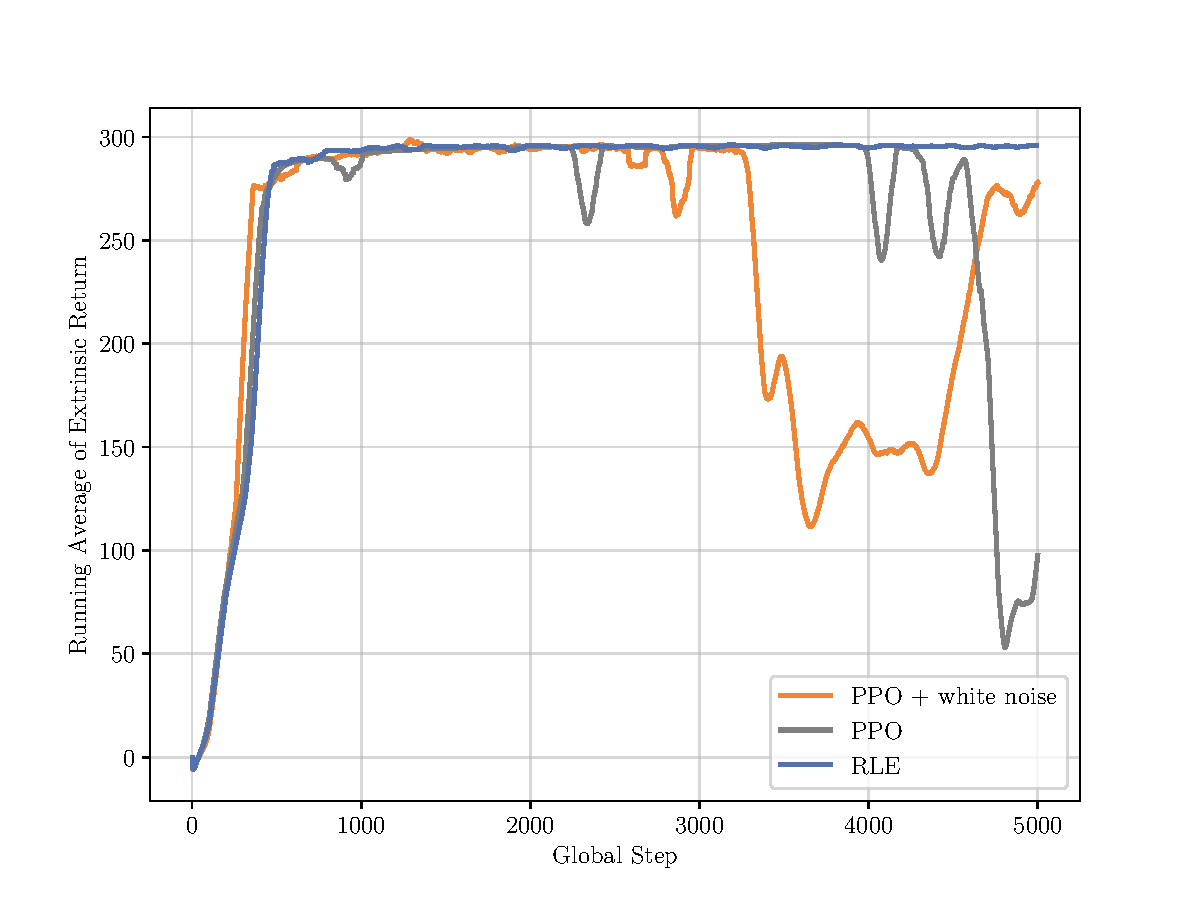
\includegraphics[width=\textwidth]{figures/plot_Cartpole_Extrinsic Return.pdf}
  \caption{\textsc{CartPole} Extrinsic Returns.}
  \label{fig:cartpole-return}
\end{figure}

\hypertarget{appendix-difficult}{\section{Difficulties}}

\noindent A major challenge we faced was evaluating \textsc{RLE} across three distinct environments, each presenting unique difficulties. For the \textsc{FourRoom} environment, no implementation was available, requiring us to develop one from scratch. We aimed to replicate the approach used by \cite{rle-paper} as closely as possible to ensure comparability. The \textsc{Atari} environment, on the other hand, could be used without modification, but training agents demanded substantial computational resources. Furthermore, in the paper, an important implementation detail, the split critic's head, is omitted. The paper itself also contains some contradicting information (\textsc{Atari} feature network size, condition to resample $\textbf{z}$) and minor errors (\textsc{FourRoom} environment description and typo in pseudocode regarding feature network update). Lastly, as \textsc{RLE} builds upon \textsc{PPO} with optimizations such as generalized advantage estimation, we had to dedicate considerable time to thoroughly understand the underlying \textsc{PPO} framework.

\noindent There are not many documentation neither active blogs about \textsc{IsaacLab}, which it makes the migration highly difficult considering the higher complexity with respect
to \textsc{IsaacGym}. In addition, the deprication of \textsc{IsaacGym} generates uncompatibilities with pre installed cuda libraries in providers as Lambda or Google which requires uninstalling
and installing older versions which can generate other issues with other pre installed libraries or requires a high amount of time debugging NVIDIA related issues.